\documentclass[a4paper,11pt,bibliography=totoc,listof=totoc,headinclude=true,cleardoublepage=empty,oneside]{scrbook}
% Option "oneside" für einseitigen Druck. Weglassen, falls die Arbeit doppelseitig gedruckt wird

\usepackage[english,ngerman]{babel}
\usepackage[utf8]{inputenc}
%\usepackage{fullpage}
\usepackage{ifthen}
\usepackage{xcolor}
\usepackage{amsmath,amsthm,amssymb,amsfonts}
\usepackage{dsfont}
\usepackage{graphicx}
\usepackage{psfrag}
\usepackage{pgfplots}
\usepackage{subcaption}
\pgfplotsset{compat=1.18}

\usepackage[T1]{fontenc}
\renewcommand{\familydefault}{cmss} % Schriftart
\newcommand{\norm}[1]{\left\lVert #1 \right\rVert}

\newtheorem{theorem}{Satz}
\newtheorem{lemma}[theorem]{Lemma}
\newtheorem{corollary}[theorem]{Korollar}
\newtheorem{satz}[theorem]{Satz}

\theoremstyle{definition}
\newtheorem{definition}[theorem]{Definition}
\newtheorem{beispiel}[theorem]{Beispiel}
\newtheorem{bemerkung}[theorem]{Bemerkung}

\theoremstyle{remark}
\newtheorem{remark}[theorem]{Bemerkung}


\definecolor{uhh_red}{RGB}{226,0,26}
\definecolor{uhh_blue}{RGB}{2,113,187}
\definecolor{uhh_grey}{RGB}{59,81,91}

\definecolor{change}{RGB}{2,113,187}

\def\revision#1{{\color{uhh_red}#1}}

\graphicspath{{../bilder/}}

% links in pdf
\usepackage{hyperref}

\hypersetup{
    colorlinks=true,
    linkcolor=orange,
    citecolor=orange,
    filecolor=orange,      
    urlcolor=purple,
    unicode,
    }


% Zum Druck verwende schwarze Links!
%\usepackage[unicode,colorlinks=true,linkcolor=black,citecolor=black,urlcolor=black,pagebackref=false]{hyperref} 
	% colorlinks=false umrahmt Links statt einzufaerben, 


% document style
\KOMAoptions{footinclude=false} % Fusszeile wird nicht zu Satzspiegel gezaehlt
\KOMAoptions{headsepline=true} % Trennlinie zwischen Kopfzeile und Text
\KOMAoptions{DIV=12} % beeinflusst Satzspiegel
\KOMAoptions{BCOR=8mm} % Bindekorrektur
\pagestyle{headings} % mit Kopfzeilen

\recalctypearea % berechne Satzspiegel neu


%%%%%%%%%%%%%%%%%%%%%%%%%%%%%%%%%%%%%%%%%%%%%%%%%%%%%%%%%%%%%%%%%%%%%%%%%%%%%%%%%%%%%%%%%%%%%%%%%%%%%%%%%%%%%%
%%%%%%%%%%%%%%%%%%%%%%%%%%%%%%%%%%%%%%%%%%%%%%%%%%%%%%%%%%%%%%%%%%%%%%%%%%%%%%%%%%%%%%%%%%%%%%%%%%%%%%%%%%%%%%
%%%%%%%%%%%%%%%%%%%%%%%%%%%%%%%%%%%%%%%%%%%%%%%%%%%%%%%%%%%%%%%%%%%%%%%%%%%%%%%%%%%%%%%%%%%%%%%%%%%%%%%%%%%%%%
%%%%%%%%%%%%%%%%%%%%%%%%%%%%%%%%%%%%%%%%%%%%%%%%%%%%%%%%%%%%%%%%%%%%%%%%%%%%%%%%%%%%%%%%%%%%%%%%%%%%%%%%%%%%%%

\begin{document}

%%%%%%%%%%%%%%%%%%%%%%%%%%%%%%%%%%%%%%%%%%%%%%%%%%%%%%%%%%%%%%%%%%%%%%%%%%%%%%%%%%%%%%%%%%%%%%%%%%%%%%%%%%%%%%
% TITELSEITE [OBLIGATORISCH]
%%%%%%%%%%%%%%%%%%%%%%%%%%%%%%%%%%%%%%%%%%%%%%%%%%%%%%%%%%%%%%%%%%%%%%%%%%%%%%%%%%%%%%%%%%%%%%%%%%%%%%%%%%%%%%

\pagenumbering{Alph}
\selectlanguage{english} %\selectlanguage{ngerman}

\begin{titlepage}
  %\vspace*{-2cm}
  \begin{center}
    
\includegraphics[width=0.45\textwidth]{uhh-logo.png}
    \vskip 1cm%
    {\LARGE B~\Large A~C~H~E~L~O~R~A~R~B~E~I~T}
    \vskip 8mm
    {\huge\bfseries\color{change}Wavelet and Fourier Transform Methods for ECG Signal}  %\[1ex] ggf.\ mehrzeilig}
    \vskip 1cm
    \large 
    ausgef\"uhrt am    
    \vskip 0.75cm
    {\Large Fachbereich Mathematik}\\[1ex]
    {\Large Fakultät für Mathematik, Informatik und Naturwissenschaften}\\[1ex]
    {\Large Universität Hamburg}
    \vskip0.75cm
    unter der Anleitung von
    \vskip0.75cm
    {\Large\bfseries\color{change}Philip Lederer}\\[1ex]
    \vskip 0.5cm
    durch
    \vskip 0.5cm
    {\Large\bfseries\color{change}Hilda Beuting}\\[1ex]
    Matrikelnummer: {\color{change}7332108}\\[1ex]
    {\color{change}Weindorfer Str. 10}\\[1ex]
    {\color{change}82418 Murnau am Staffelsee}
  \end{center}
  
  \vfill
  
  \small
  Hamburg, am {\color{change} Datum} %\today
  \vspace*{-15mm}
\end{titlepage}

\cleardoublepage

%%%%%%%%%%%%%%%%%%%%%%%%%%%%%%%%%%%%%%%%%%%%%%%%%%%%%%%%%%%%%%%%%%%%%%%%%%%%%%%%%%%%%%%%%%%%%%%%%%%%%%%%%%%%%%
% DANKSAGUNG / ACKNOWLEDGEMENT [OPTIONAL]
%%%%%%%%%%%%%%%%%%%%%%%%%%%%%%%%%%%%%%%%%%%%%%%%%%%%%%%%%%%%%%%%%%%%%%%%%%%%%%%%%%%%%%%%%%%%%%%%%%%%%%%%%%%%%%

\chapter*{Acknowledgement} %\chapter*{Danksagung}
\thispagestyle{empty}
\selectlanguage{english} %\selectlanguage{ngerman}

{\color{change}
\begin{itemize}
\item auf Deutsch oder Englisch
\item Die Danksagung (engl. {\em Acknowledgement}) ist optional und kann auch entfallen. Denken Sie ggf.\ an Ihre eigenen Eltern! danken an alle blahblah

\item Falls die Arbeit durch eine Forschungsprojekt finanziert wurde, so ist jedenfalls der Fördergeber (z.B. DFG...) mit Projektnummer und Projektname zu nennen.

\end{itemize}
}

\cleardoublepage

% %%%%%%%%%%%%%%%%%%%%%%%%%%%%%%%%%%%%%%%%%%%%%%%%%%%%%%%%%%%%%%%%%%%%%%%%%%%%%%%%%%%%%%%%%%%%%%%%%%%%%%%%%%%%%%
% % EIDESSTATTLICHE ERKLAERUNG [OBLIGATORISCH]
% %%%%%%%%%%%%%%%%%%%%%%%%%%%%%%%%%%%%%%%%%%%%%%%%%%%%%%%%%%%%%%%%%%%%%%%%%%%%%%%%%%%%%%%%%%%%%%%%%%%%%%%%%%%%%%

% \chapter*{Eidesstattliche Erkl\"arung}
% \thispagestyle{empty}
% \selectlanguage{ngerman}
% \thispagestyle{empty}

% \vspace*{2cm}

% Ich erkl\"are an Eides statt, dass ich die vorliegende Bachelorarbeit selbstst\"andig und ohne fremde Hilfe verfasst, andere als die angegebenen Quellen und Hilfsmittel nicht benutzt bzw. die w\"ortlich oder sinngem\"a{\ss} entnommenen Stellen als solche kenntlich gemacht habe.

% \vspace*{3cm}

% \noindent
% Hamburg, am {\color{change}Datum} %\today
% %
% \hfill 
% %
% \begin{minipage}[t]{5cm}
% \centering
% \underline{\hspace*{5cm}}\
% \small\color{change}Name des Autors
% \end{minipage}

% \cleardoublepage

%%%%%%%%%%%%%%%%%%%%%%%%%%%%%%%%%%%%%%%%%%%%%%%%%%%%%%%%%%%%%%%%%%%%%%%%%%%%%%%%%%%%%%%%%%%%%%%%%%%%%%%%%%%%%%
% INHALTSVERZEICHNIS [OBLIGATORISCH]
%%%%%%%%%%%%%%%%%%%%%%%%%%%%%%%%%%%%%%%%%%%%%%%%%%%%%%%%%%%%%%%%%%%%%%%%%%%%%%%%%%%%%%%%%%%%%%%%%%%%%%%%%%%%%%

\pagenumbering{roman}
\selectlanguage{ngerman} %\selectlanguage{english}  

\tableofcontents

\cleardoublepage
\pagenumbering{arabic} 

%%%%%%%%%%%%%%%%%%%%%%%%%%%%%%%%%%%%%%%%%%%%%%%%%%%%%%%%%%%%%%%%%%%%%%%%%%%%%%%%%%%%%%%%%%%%%%%%%%%%%%%%%%%%%%
% EINLEITUNG / INTRODUCTION [OBLIGATORISCH]
%%%%%%%%%%%%%%%%%%%%%%%%%%%%%%%%%%%%%%%%%%%%%%%%%%%%%%%%%%%%%%%%%%%%%%%%%%%%%%%%%%%%%%%%%%%%%%%%%%%%%%%%%%%%%%

%%%%%%%%%%%%%%%%%%%%%%%%%%%%%%%%%%%%%%%%%%%%%%%%%%%%%%%%%%%%%%%%%%%%%%%%%%%%%%%%%%%%%%%%%%%%%%%%%%%%%%%%%%%%%%
%%%%%%%%%%%%%%%%%%%%%%%%%%%%%%%%%%%%%%%%%%%%%%%%%%%%%%%%%%%%%%%%%%%%%%%%%%%%%%%%%%%%%%%%%%%%%%%%%%%%%%%%%%%%%%
%\chapter{inoffizielles Inhaltsverzeichnis}
%\noindent 
%hier die aktuelle Idee/Planung 
%\
%\ Thema: Wavelettransformation of EKG signals
%\
%\ 1. Einleitung 
%\ Die (diskrete) Wavelet und Fourier Transformation wird ja insbesondere im Bereich von Signal-Analysen verwendet. Dabei geht es darum ein Signal von Störungen (Rauschen) zu befreien. Mit lokalen Störungen kann die Wavelettransformation besser als die Fourier-Transformation umgehen. Was ich dabei explizit im Kopf habe sind EKG Signale. Die Arbeit könnte sich also zuerst mit den Grundlagen von Wavelets beschäftigen (und auch der Fourier Transformation). Dort können Sie auch nochmal explizit Konvergenzaussagen besprechen etc… Dann diskutieren sie die diskrete Wavelettrafo, implementieren diese, und wenden Sie dann auf “echte” Signale an. Für EKG Signale gibt es zugängliche Datensätze (googlen Sie mal MIT-BIH).
%\Grundlage Signalanalyse, Wie ensteht rasuchen? warum will man das vermeiden? Beide Methoden kurz anreissen. 
%%\ Literatur: 
%\
%\ 2. mathematische Grundlagen - stellt sich dann später heraus was genau man da braucht - alles aufschreiben was ich zuerst nciht sofort verstehe 
%\ $L^2$ Raum, Hilberträume, Orthonormalbasen
%\ Literatur: 
%\
%\ 3. Fourier Transformation 
%\ 3.1 Theorie 
%\ 3.2 Konvergenzaussagen 
%\ 3.3 denoising mit Fouriertransformation 
%\
%\ Literatur: Fourier Analysis/ An Introduction - Elias M. Stein, Rami Shakarchi;
%\ Fourier Analysis and Its Applications - G. B. Folland; 
%\            
%\
%\ 4. wavelets 
%\ 4.1 Theorie - haar wavelet, beweis orthognoalität haar-basis in $L^2$, Mulitresolution analysis
%\ 4.2 Konvergenzaussagen 
%\ 4.3 denoising mit wavelettransformation
%\ Literatur: Ingrid Daubechies: Ten lectures on wavelets.
%\
%\ 5 . Anwendung auf EKG Signale 
%\ 5.1 Datensätze und Vorbereitung
%\ 5.2 Implementierung der Wavelettransformation mit fouriertransformation
%\ 5.3 Implementierung der Wavelettransformation mit diskreter wavelettransformation - vll mit unterschiedlichen wavelets (Haar, Daubechies, Symlet, ...)
%\ 5.4 Ergebnisse und Auswertung - Vor und Nachteile, Beobachtungen, Grenzen was geht immer noch nicht?
%\ Literatur:
%\
%\  6. conclusion
%\ Zusammenfassung der wichtigsten Punkte 
%
%
\chapter{Introduction}
\label{chapter:introduction}
%%%%%%%%%%%%%%%%%%%%%%%%%%%%%%%%%%%%%%%%%%%%%%%%%%%%%%%%%%%%%%%%%%%%%%%%%%%%%%%%%%%%%%%%%%%%%%%%%%%%%%%%%%%%%%
%%%%%%%%%%%%%%%%%%%%%%%%%%%%%%%%%%%%%%%%%%%%%%%%%%%%%%%%%%%%%%%%%%%%%%%%%%%%%%%%%%%%%%%%%%%%%%%%%%%%%%%%%%%%%%

{\color{change}

\noindent 
\begin{itemize}
  \item EKG Daten sind verauscht z.B durch Bewegungsartefakte, Störungen durch andere Geräte, ... für die richtige Interpretatiion der Signale ist es wichtig, diese Störungen zu entfernen. 
  \item Es gibt verschiedene Möglichkeiten, um das Rauschen zu entfernen. Eine Möglichkeit ist die Fourier-Transformation, eine andere Möglichkeit ist die Wavelet-Transformation.
  \item Diese Arbeit soll die mathematischen Hintergründe der Fourier- und Wavelet-Transformation erläutern und dann die Anwendung auf EKG Signale diskutieren.
\end{itemize}

}


%%%%%%%%%%%%%%%%%%%%%%%%%%%%%%%%%%%%%%%%%%%%%%%%%%%%%%%%%%%%%%%%%%%%%%%%%%%%%%%%%%%%%%%%%%%%%%%%%%%%%%%%%%%%%%
\chapter{Mathematical Foundations}
\label{chapter:content}

\section{Der $L^2$ Raum}

\begin{definition}{$L^2$-Norm} \cite[S.35, Abschnitt 2.2]{blatterWaveletsEinfuhrung2003}
  Sei $f:\mathbb{R} \to \mathbb{C}$ eine messbare Funktion, die $2\pi$-periodisch ist. 
  Dann ist die \textbf{$L^2$-Norm} von $f$, definiert als: 
  \[  
  \norm{f}_{L^2} := \sqrt{\left\langle f, f \right\rangle} = (\frac{1}{2\pi} \int_{0}^{2\pi} |f(t)|^2 dt)^{1/2}
  \]
\end{definition}


Im folgenden gelte die Konvention, damit man nicht so oft schreiben muss,

\[ 
\norm{f} := \norm{f}_{L^2}
\]

\begin{itemize}
\item $L^1$
\item $L^2$
\item faltungssatz für umkehreformel - kapitel
\item Hilberträume
\item Orthonormalbasen
\end{itemize}

die Zulässigkeitskonstante aus Definition 2 (2) von $\psi$ ist und $H := L^2(\mathbb{R}^2_-, d\mu)$
   mit dem Maß $d\mu = \frac{da\,db}{|a|^2}$.

   WAS IST DIESES MAß UND WAS IST R2- MUSS IN GRUNDLAGEN

%%%%%%%%%%%%%%%%%%%%%%%%%%%%%%%%%%%%%%%%%%%%%%%%%%%%%%%%%%%%%%%%%%%%%%%%%%%%%%%%%%%%%%%%%%%%%%%%%%%%%%%%%%%%%%





\chapter{Fourier Transform}

%%%%%%%%%%%%%%%%%%%%%%%%%%%%%%%%%%%%%%%%%%%%%%%%%%%%%%%%%%%%%%%%%%%%%%%%%%%%%%%%%%%%%%%%%%%%%%%%%%%%%%%%%%%%%%
\section{Theoretical foundations}

 \subsection{Fourier series} % fourier reihe
  was ist die fourierreihe wie entstehen die koeffzienten
  \cite[Chapter 5, Section 1.1]{steinFourierAnalysisIntroduction2003a}
  \cite[Definition 2.1]{serovFourierSeriesFourier2017} und folgende Seite

 \subsection{Definition of the Fourier Transform} % kontinuierliche ft mit $f \in L^1(\mathbb{R})$ dann erweitern
 auf $M(\mathbb{R})$
  \cite[Chapter 5, Section 1.2]{steinFourierAnalysisIntroduction2003a}
 
 \subsection{Definition of the Schwarz space} 
  f in S -> f in $L^2$ -> vll dann besser in grundlagen 
  \cite[Chapter 5, Section 1.3]{steinFourierAnalysisIntroduction2003a}
  \cite[Definition 16.1]{serovFourierSeriesFourier2017}

 \subsection{Fourier Transform on the Schwarz space} 
  \cite[Chapter 5, Section 1.4]{steinFourierAnalysisIntroduction2003a}
  \cite[Definition 16.5]{serovFourierSeriesFourier2017}

 \subsection{Properties of the Fourier Transform} % eigenschaften: lineaität, translation, skalierung
  \cite[page 136, definition 16.8]{serovFourierSeriesFourier2017} 

 \subsection{Convolution Theorem of the Fourier Transform}
  \cite[Chapter 2, Section 3]{steinFourierAnalysisIntroduction2003a}
  \cite[Chapter 2, Proposition 3.1]{steinFourierAnalysisIntroduction2003a}
  \cite[S.32, 33]{cooleyFastFourierTransform1969} 

 \subsection{Inverse Fourier Transform} % definitione der inversen
  \cite[Chapter 5, Section 1.5]{steinFourierAnalysisIntroduction2003a}
  \cite[Chapter 5, Theorem 1.9 - Fourier Inversion]{steinFourierAnalysisIntroduction2003a} % fourier inversionstheorem($L^1$)
  oder \cite[Theorem 16.10 - Fourier Inversion]{serovFourierSeriesFourier2017}

 \subsection{Plancherel Theorem} % plancherel theorem/ isometrie auf $L^2$
  \cite[Chapter 5, Section 1.6]{steinFourierAnalysisIntroduction2003a}
  \cite[Chapter 5, Theorem 1.12]{steinFourierAnalysisIntroduction2003a}
  \cite[Theorem 17.5 - Plancherel Theorem]{serovFourierSeriesFourier2017}

 \subsection{The windowed FOurier Transform}


 \subsection{Discrete Fourier Transform} % diskrete ft mit komplexität $\mathcal{O}(N^2)$
  \cite[Chapter 11, introduchtion]{serovFourierSeriesFourier2017}
  \cite[Definition 11.1]{serovFourierSeriesFourier2017} %DFT
  \cite[Definition 11.2]{serovFourierSeriesFourier2017} %IDFT
  \cite[Corollary 11.4]{serovFourierSeriesFourier2017} %Parsevalsche Gleichung für DFT
  \cite[Definition 11.7]{serovFourierSeriesFourier2017} %convolution of discrete sequences 
  auch alles in \cite[S.28]{cooleyFastFourierTransform1969}

 \subsection{Fast Fourier Transform} % fast fourire transform mit komplexität $\mathcal{O}(N * \log N)$
 % muss noch seite raussuchen

\section{Convergence results}
 \subsection{Mean square convergence of Fourier series} 
  \cite[Chapter 3, Theorem 1.1]{steinFourierAnalysisIntroduction2003a}
  
 \subsection{Convergence of Fourier series in $L^1$}
  \cite[Chapter 2, Theorem 5.2]{steinFourierAnalysisIntroduction2003a} %erklärung s. 51-54

 \subsection{Convergence of Fourier series in $L^2$}
  \cite[Chapter 3, Theorem 2.1]{steinFourierAnalysisIntroduction2003a} %erklärung s. 51-54

 \subsection{COnvergence of the Windowed Fourier Transform} 

 %evtl. punktweise konvergenz - man vermeidet die? warum?
 % -> gegenbeispiel: stetige fkt mir divergenter fourier reihe - siehe \cite[Chapter 3, S. 83-87]{steinFourierAnalysisIntroduction2003a} 
 % dirichlet kernel - bedingung für punktweise/uniforme konvergenz 

\section{Denoising/ Signal Processing with Fourier Transform} %theorie dahinter

signalmodell: signal = signal + rauschen


idee: im frequenzenbereich sind signal und rauschen oft trennbar


faltungssatz der fourier transform: im frequenzbereich wird faltung zu multiplikation - spektrales filtern
-> übertragen von convolution theorem von vorher - maybe faltungssatz schon mal ganz oben.


digitales filtern: \cite[S. 33]{cooleyFastFourierTransform1969}


filtertypen: low-pass, high-pass, band-pass, band-stop -> noch nichtsgenaues rausgesucht 


thresholding: hard thresholding, soft thresholding -> auch noch nichts genaues rausgesucht 


hier schon konkrete anwedung auf ekg signale? oder lieber erst wavelet theorie und dann einführung ekg und dann erst fourier und dann wavelet?
-> theorie ecg interpretation aber dann muss man fast unterkapitel erstellen....

hier leichtes beispiel

rauschen eienmal global mit cos einmal lokal mit gauss - dann fourier transformieren und schauen was passiert - vll auch mit fensterung - aber dann muss ich ja fenstergröße festlegen - das ist ja auch wieder problematisch - siehe heisenberg'sche unschärferelation



\section{Limitations of Fourier Transform for Denoising}
 \subsection{heisenberg uncertainty principle} %übergang von fourier zu wavelet -> hier betonung auf warum fourier deswegen nciht gut funkntioniert
  \cite[Chapter 5, Section 4]{steinFourierAnalysisIntroduction2003a} %erklärung 
  \cite[Chapter 5, Theorem 4.1]{steinFourierAnalysisIntroduction2003a} %grundlage warum ft nciht lokal sondern global ist

% ft setzt voraus, dass das signal keine zeitlichen variationen hat, d.h. es ist nicht gut geeignet für signale mit lokalen störungen
% man kann nicht genau sagen, wo im signal die störungen auftreten, da die ft global ist - heisenberg'sche unschärferelation
% ecg signals haben oft lokale störungen, z.b. durch bewegungsartefakte, die ft nicht gut entfernen kann -> schlecht
% vll gefensterte FT - aber dann feste fenstergröße dh. festes zeit-frequenz-aufteilung - muss ich gefensterte Ft machen? 
% wavelet transform bietet hier eine bessere alternative, da sie lokal ist und somit besser mit lokalen störungen umgehen kann

%%%%%%%%%%%%%%%%%%%%%%%%%%%%%%%%%%%%%%%%%%%%%%%%%%%%%%%%%%%%%%%%%%%%%%%%%%%%%%%%%%%%%%%%%%%%%%%%%%%%%%%%%%%%%%
%%%%%%%%%%%%%%%%%%%%%%%%%%%%%%%%%%%%%%%%%%%%%%%%%%%%%%%%%%%%%%%%%%%%%%%%%%%%%%%%%%%%%%%%%%%%%%%%%%%%%%%%%%%%%%


\chapter{Wavelet Transform}

% Literatur gesamt:
% \cite{mallatWaveletTourSignal1999}
% \cite{gacekIntroductionECGSignal2012}
% \cite{blatterWaveletsEinfuhrung2003}
% \cite{daubechiesTenLecturesWavelets2006}

% ============================================================

\section{Motivation – Übergang von Fourier zu Wavelet}
  % \cite[S. 25, 34]{gacekIntroductionECGSignal2012}
  % \cite[p. vii]{daubechiesTenLecturesWavelets2006}
  % \cite[S. 8, 9]{blatterWaveletsEinfuhrung2003}
  % \cite[S. 10--12]{blatterWaveletsEinfuhrung2003}
  % \cite[S. 433]{hanke-bourgeoisGrundlagenNumerischenMathematik2009}

  \begin{itemize}
    \item Fourier-Transformation: global, zeigt \emph{was} an Frequenzen vorhanden,
      aber nicht \emph{wann} \cite[S.\,8, 9]{blatterWaveletsEinfuhrung2003}
    \item EKG hat abrupte, lokale Ereignisse (QRS-Komplex) → Lokalität ist entscheidend
      \cite[S.\,25, 34]{gacekIntroductionECGSignal2012}
    \item Kurzzeit-Fouriertransformation (STFT / WFT)
      \cite[S.\,10--12]{blatterWaveletsEinfuhrung2003}:
      \begin{itemize}
        \item bietet Lokalität durch Fensterfunktion
        \item aber: Fensterbreite fix → schlechter Kompromiss zwischen Zeit- und Frequenzauflösung
      \end{itemize}
    \item Lösung: Wavelet-Transformation mit adaptiver Fensterbreite
      \cite[p.\,vii]{daubechiesTenLecturesWavelets2006}
    \item nicht mehr trigonometrische Polynome als basis, wie bei fourier 
    -> weil schlechte lokalisierungseigenschaft 
    -> aber wir wollen die eigenschaft eine gute frequenzanalyse zu bekommen behalten 
    -> aber: mit örtlicher lokalisierung
    -> multiskalenbasen: andere basis wählen nämlich: wavelets  
  \end{itemize}

  % ------------------------------------------------------------
  %\subsection{Wavelet-Transformation (Überblick / Intuition)}
  %% \cite[Section 1.5]{blatterWaveletsEinfuhrung2003}
  %wavelet heisst kleine welle
  %\begin{itemize}
  %  \item Ziel: Signal $f\colon \mathbb{R} \to \mathbb{C}$ simultan in Zeit \emph{und} Frequenz
  %    analysieren \cite[Section~1.5]{blatterWaveletsEinfuhrung2003}
  %  \item \textbf{Mutterwavelet} $\psi$ mit kompaktem Träger $[0,L]$
  %  \item \textbf{Waveletfunktion} durch Skalierung ($a$) und Verschiebung ($b$):
  %    \[
  %      \psi_{a,b}(t) = \frac{1}{|a|^{1/2}}\,\psi\!\left(\frac{t-b}{a}\right),
  %      \quad a \in \mathbb{R}^*, \; b \in \mathbb{R}
  %    \]
  %  \item $|a| \gg 1$: breites Fenster → langwellige / niederfrequente Anteile
  %  \item $0 < |a| \ll 1$: schmales Fenster → hochfrequente / kurzlebige Anteile
  %  \item \textbf{BILD} analog zu \cite[S.\,15]{blatterWaveletsEinfuhrung2003} einfügen
  %  \item \textbf{Wavelet-Transformierte} $Wf\colon \mathbb{R}^* \times \mathbb{R} \to \mathbb{C}$:
  %    \[
  %      Wf(a,b) := \langle f, \psi_{a,b} \rangle
  %               = \frac{1}{|a|^{1/2}} \int_{-\infty}^{\infty}
  %                 f(t)\,\overline{\psi\!\left(\frac{t-b}{a}\right)}\,dt
  %    \]
  %  \item \textbf{Umkehrformel} (Rekonstruktion):
  %    \[
  %      f = \frac{1}{C_{\psi}} \int_{\mathbb{R}^* \times \mathbb{R}}
  %          \frac{da\,db}{|a|^2}\, Wf(a,b)\,\psi_{a,b}
  %    \]
  %    \begin{itemize}
  %      \item $f$ als Linearkombination der Basisfunktionen $\psi_{a,b}$
  %      \item $C_{\psi}$ hängt vom gewählten Mutterwavelet ab (Admissibility-Konstante)
  %    \end{itemize}
  %  \item \textbf{Anforderungen an das Mutterwavelet $\psi$}:
  %    \begin{itemize}
  %      \item $\psi \in L^1(\mathbb{R}) \cap L^2(\mathbb{R})$
  %      \item Nullmittelbedingung: $\int_{-\infty}^{\infty} \psi(t)\,dt = 0$
  %      \item Admissibilitätsbedingung: $C_{\psi} = \int_0^\infty \frac{|\hat\psi(\omega)|^2}{\omega}\,d\omega < \infty$
  %      \item Relativ freie Wählbarkeit im Vergleich zur Fourier-Transformation
  %    \end{itemize}
  %  \item Einfachstes einführendes Beispiel: Haar-Wavelet (s.\,nächster Abschnitt)
  %\end{itemize}
%
  %% ------------------------------------------------------------
  %\subsection{Haar-Wavelet}
  %\begin{itemize}
  %  \item Definition:
  %    \[
  %      \psi_{\mathrm{Haar}}(x) :=
  %      \begin{cases}
  %        \phantom{-}1  & x \in [0, \tfrac{1}{2}), \\
  %        -1            & x \in [\tfrac{1}{2}, 1], \\
  %        \phantom{-}0  & \text{sonst.}
  %      \end{cases}
  %    \]
  %  \item Träger: $[0,1]$, kompakt
  %  \item Eigenschaften:
  %    \begin{itemize}
  %      \item $\int_{-\infty}^{\infty} \psi_{\mathrm{Haar}}(x)\,dx = 0$
  %      \item $\|\psi_{\mathrm{Haar}}\|_{L^2}^2 = 1$
  %      \item Gut im Zeitbereich lokalisiert (kleiner Träger)
  %      \item Nachteil: unstetig (Sprungstellen) → schlechte Frequenzlokalisation
  %    \end{itemize}
  %  \item \textbf{Waveletfunktionen} (Skalierungs- und Verschiebungsindizes $r, k \in \mathbb{Z}$):
  %    \[
  %      \psi_{r,k}(t) := 2^{-r/2}\,\psi_{\mathrm{Haar}}\!\left(\frac{t - k \cdot 2^r}{2^r}\right),
  %      \quad \text{Träger } I_{r,k} = [k \cdot 2^r,\,(k+1) \cdot 2^r)
  %    \]
  %    \begin{itemize}
  %      \item Trägerlänge $2^r$: größeres $r$ → langwelligeres $\psi_{r,k}$
  %      \item Normierungsfaktor $2^{-r/2}$ sichert $\|\psi_{r,k}\|^2 = 1$ für alle $r,k$
  %      \item Kleinere Intervalle → größere Amplitude; größere Intervalle → kleinere Amplitude
  %    \end{itemize}
%
  %  \item \textbf{Satz (Orthonormalbasis):} $\{\psi_{r,k} \mid r,k \in \mathbb{Z}\}$ ist
  %    Orthonormalbasis von $L^2(\mathbb{R})$
  %    \cite[prop.~56.2]{hanke-bourgeoisGrundlagenNumerischenMathematik2009}
%
  %  \item \textbf{Beweis – Orthonormalität} ($\langle \psi_{r,k}, \psi_{s,l}\rangle = \delta_{r,s}\delta_{k,l}$):
  %    \begin{itemize}
  %      \item \textbf{Fall 1} ($r = s$, $k \neq l$): Träger $I_{r,k}$ und $I_{r,l}$ disjunkt
  %        → Integral über disjunkte Träger = 0
  %      \item \textbf{Fall 2} ($s < r$, o.\,B.\,d.\,A.): $I_{r,k}$ liegt ganz in linker oder rechter
  %        Hälfte von $I_{s,l}$ → $\psi_{s,l}$ ist auf $I_{r,k}$ konstant $c$
  %        → $\langle \psi_{r,k}, \psi_{s,l}\rangle = c \int_{I_{r,k}} \psi_{r,k} = 0$,
  %        da $\int \psi_{r,k} = 0$
  %      \item \textbf{Normierung}: $\|\psi_{r,k}\|^2 = 1$ per Konstruktion des Faktors $2^{-r/2}$
  %    \end{itemize}
%
  %  \item \textbf{Beweis – Vollständigkeit} (das ONS ist eine Basis)
  %    \cite[Abschnitt~1.6, S.\,20--24]{blatterWaveletsEinfuhrung2003}:
  %    \begin{itemize}
  %      \item Strategie: erst für Treppenfunktionen mit kompaktem Träger zeigen, dann allgemein
  %        \begin{itemize}
  %          \item Treppenfunktionen mit kompaktem Träger liegen dicht in $L^2(\mathbb{R})$
  %            (Verweis: Satz aus Funktionalanalysis, noch einfügen)
  %        \end{itemize}
  %      \item \textbf{Verdopplungsverfahren / Induktion}:
  %        Grundidee: $f$ wird durch immer feinere Schichten von Waveletpolynomen approximiert;
  %        man startet grob und fügt Schritt für Schritt feinere Details hinzu
  %      \item Waveletpolynom auf Ebene $r$:
  %        $\psi_r := \sum_{j=-n+1}^{r} \sum_k c_{j,k}\,\psi_{j,k}$
  %      \item Rest: $f_r := f - \psi_r$, konstant auf $I_{r,k}$
  %        (Wert = Mittelwert von $f$ auf $I_{r,k}$)
  %        \begin{itemize}
  %          \item TODO: Begründung einfügen, warum $f_r$ konstant auf $I_{r,k}$ ist
  %        \end{itemize}
  %      \item \textbf{Induktionsanfang} ($r = -n$):
  %        $\psi_{-n} := 0,\quad f_{-n} := f$
  %      \item \textbf{Induktionsschritt} ($r \to r' := r+1$):
  %        \begin{align*}
  %          \delta_{r',k}   &:= \tfrac{1}{2}(f_{r,2k} - f_{r,2k+1}), \\
  %          f_{r',k}        &:= \tfrac{1}{2}(f_{r,2k} + f_{r,2k+1}), \\
  %          c_{r',k}        &:= 2^{r'/2}\,\delta_{r',k}, \\
  %          \psi_{r'}       &:= \psi_r + \sum_k c_{r',k}\,\psi_{r',k}
  %        \end{align*}
  %        → TODO: Formel für $\psi_{r'}$ noch vervollständigen / prüfen
  %      \item Mit $r \to \infty$ gilt $\|f_r\|_{L^2} \to 0$, da Treppenfunktion mit
  %        immer feinerem Gitter gegen $f$ konvergiert
  %    \end{itemize}
%
  %  \item \textbf{Hinweise / Ausblick aus dem Beweis}:
  %    \begin{itemize}
  %      \item Der Induktionsschritt liefert bereits eine effiziente Berechnung der Koeffizienten
  %        → Vorläufer des schnellen Algorithmus (Mallat)
  %      \item Das Verdopplungsverfahren ist keine Besonderheit des Haar-Wavelets, sondern gilt
  %        für alle Mutterwavelets, die eine Multiskalenanalyse (MRA) zulassen → Überleitung zu MRA
  %      \item Ergänzung: Approximation einer konkreten Funktion durch Haar-Wavelets
  %        \cite[S.\,23--24]{blatterWaveletsEinfuhrung2003} – sinnvoll wegen EKG-Bezug
  %    \end{itemize}
  %\end{itemize}
%
  %% ------------------------------------------------------------
  %\subsection{Heisenbergsche Unschärferelation für die Wavelet-Transformation}
  %% \cite[Section 2.3]{blatterWaveletsEinfuhrung2003}
  %% \cite[p. 107]{daubechiesTenLecturesWavelets2006}
  %\begin{itemize}
  %  \item Prinzip: Zeit- und Frequenzauflösung können nicht gleichzeitig beliebig gut sein
  %    \cite[Section~2.3]{blatterWaveletsEinfuhrung2003}
  %    \cite[p.\,107]{daubechiesTenLecturesWavelets2006}
  %  \item Quantitative Formulierung der Unschärferelation für $\psi_{a,b}$:
  %    \begin{itemize}
  %      \item Zeitbreite $\propto |a|$, Frequenzbreite $\propto 1/|a|$
  %      \item Produkt (Zeit $\times$ Frequenz) konstant $\geq \tfrac{1}{2}$
  %    \end{itemize}
  %  \item Vorteil Wavelet ggü.\ STFT: Fensterbreite \emph{adaptiv}:
  %    \begin{itemize}
  %      \item Grobe Skalen (großes $|a|$): gute Frequenzauflösung, schlechte Zeitauflösung
  %      \item Feine Skalen (kleines $|a|$): gute Zeitauflösung, schlechte Frequenzauflösung
  %    \end{itemize}
  %  \item → Erklärung, warum Wavelets für Signale mit lokalen Ereignissen (EKG) besser als Fourier
  %  \item TODO: Prüfen ob Satz formal ausgeführt werden soll oder nur zur Motivation genutzt wird
  %\end{itemize}


% ============================================================
\section{Theoretische Grundlagen}
 hier fehlt ncohe einführender satz....!
  % ------------------------------------------------------------
\subsection{Kontinuierliche Wavelet-Transformation (CWT)}
% \cite[Section 3.1]{blatterWaveletsEinfuhrung2003}
% \cite[ch. 2, p. 17--52]{daubechiesTenLecturesWavelets2006}

\begin{definition}{Wavelet} \cite[S.~54, Section~3.1]{blatterWaveletsEinfuhrung2003}

  Ein \textbf{Wavelet} oder auch \textbf{Mutterwavelet} ist eine Funktion
  $\psi: \mathbb{R} \to \mathbb{C}$, die die folgenden Bedingungen $(1)$ und $(2)$ erfüllt:
  \[
    \psi \in L^2, \quad \norm{\psi} = 1, \tag{1}
  \]
  \[
    2\pi \int_{\mathbb{R}^*} \frac{|\hat\psi(t)|^2}{|t|} \, dt =: C_\psi < \infty, \tag{2}
  \]
  wobei $\norm{\psi}$ die $L^2$-Norm von $\psi$ (siehe Definition (2.?)) und $\hat\psi$ (wie
  gehabt) die Fourier-Transformierte von $\psi$ ist.

\end{definition}

Die erste Bedingung $(1)$ stellt sicher, dass $\psi$ in $L^2$ liegt und damit, dass
\[
  \int_{-\infty}^{\infty} |\psi(t)|^2 \, dt < \infty.
\]
Damit ist $\psi$ kein \glqq unendliches Signal\grqq, was eine notwendige Voraussetzung für
die Analyse von Signalen ist.
Die Normierung $\norm{\psi} = 1$ ist eine Konvention, die es ermöglicht, die Energie des
Signals korrekt zu interpretieren und zu vergleichen.

Die zweite Bedingung $(2)$ wird auch als Zulässigkeitsbedingung bezeichnet.
Das folgende Lemma gibt eine äquivalente Formulierung, die die Interpretation einfacher macht.

\begin{lemma} \cite[S.~54, Section~3.1]{blatterWaveletsEinfuhrung2003}

  Sei weiterhin $\psi \in L^2$ mit $t\psi \in L^1$, dann gilt:
  Die Zulässigkeitsbedingung $(2)$ ist äquivalent zu der Bedingung, dass
  \[
    \hat\psi(0) = \frac{1}{2\pi} \int_{-\infty}^{\infty} \psi(t) \, dt = 0.
  \]

\end{lemma}

\textcolor{blue}{KOMMENTAR: MUSS ICH DAS BEWEISEN? und WAS BEDEUTET $t\psi \in L^1$?? was ist t überhaupt?}

Nach Bedingung $(2)$ ist also der Mittelwert von einem Wavelet $\psi$ gleich Null, damit liegt
ein Wavelet immer teilweise über und teilweise unter der $t$-Achse und hat damit in etwa die
Form einer Welle.

Wir haben nun unser Wavelet $\psi$ definiert und damit die Rahmenbedingungen geschaffen, um
unsere Wavelet-Transformierte zu definieren.

HIER KÖNNTE MAN DAS HAAR BEISPIEL EINFÜGEN... ncoh ohne CWT sondern einfach mal bedingenugne zeigen...

\begin{definition}{Kontinuierliche Wavelet-Transformation} \cite[S.~55, Section~3.1]{blatterWaveletsEinfuhrung2003}

  Sei $f \in L^2$ und $\psi$ ein fest gewähltes Wavelet, dann ist die \textbf{kontinuierliche
  Wavelet-Transformation} von $f$ bezüglich $\psi$ definiert als:
  \[
    Wf(a,b) := \langle f, \psi_{a,b} \rangle
    = \frac{1}{|a|^{1/2}} \int_{-\infty}^{\infty} f(t)\,\overline{\psi\!\left(\frac{t-b}{a}\right)}\,dt,
  \]
  wobei $\psi_{a,b}(t) := \frac{1}{|a|^{1/2}} \psi\!\left(\frac{t-b}{a}\right)$, mit
  $a, b \in \mathbb{R},\, a \neq 0$, die skalierte und verschobene Version von $\psi$ ist.

\end{definition}

$Wf(a,b)$ misst die Ähnlichkeit von $f$ mit der Waveletfunktion $\psi_{a,b}$, die um $b$
verschoben und mit der Skala $a$ gestreckt oder gestaucht ist.
Der Faktor $\frac{1}{|a|^{1/2}}$ sorgt dafür, dass die Transformation bezüglich der $L^2$ -Norm bleibt auf 1 normiert bleibt, es gilt also 
$ ||\psi(a,b)||_{L^2} = ||\psi||_{L^2} = 1$, das $||\psi||_{L^2} = ||\psi_{a,b}||_{L^2}$ gilt kann man durch Substitution von $u= t-b/a$ sofort sehen. NACHRECHNEN


\begin{beispiel}
  \textcolor{red}{Um die neuen Definitionen einordnen zu können, hier zur Veranschaulichung ein Beispiel.}
  Betrachte das Mexikanerhut-Wavelet, welches definiert ist durch die Funktion:
  \[
    \psi(t) = \frac{2}{\sqrt{3}\,\pi^{1/4}} (1 - t^2)\, e^{-t^2/2}.
  \]

  \textcolor{blue}{EIGENTLICH MÜSSTE MAN ZEIGEN DASS DAS IN L2 UND TPSI IN L1 IST, MITTELWERT NULL IST OFFENSICHTLICH}

  Zur Veranschaulichung der Waveletfunktion $\psi_{a,b}$ betrachten wir die folgende
  Abbildung~(4.?), die die Mutterfunktion $\psi$ und zwei skalierte und verschobene Versionen
  $\psi_{a,b}$ mit unterschiedlichen Werten für $a$ und $b$ zeigt.

  \begin{figure}[htbp]
    \centering
    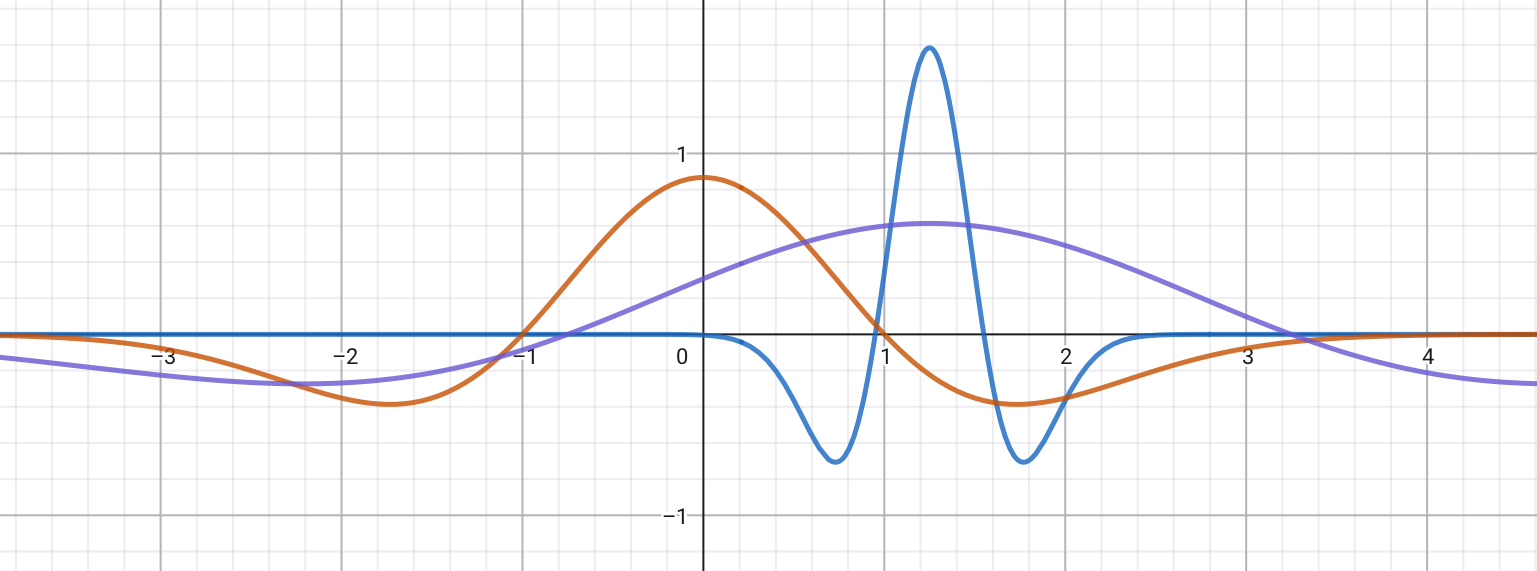
\includegraphics[width=0.8\textwidth,keepaspectratio]{mexikanerhut_verschoben.jpg}
    \caption{Das Mutterwavelet $\psi_{1,0}$ des Mexikanerhut-Wavelets in orange, sowie die
      skalierten und verschobenen Versionen $\psi_{0.3,1.25}$ in blau und $\psi_{2,1.25}$
      in lila.}
  \end{figure}

  Der Parameter $b$ verschiebt das Wavelet entlang der $t$-Achse, während der Parameter $a$
  die Breite und Höhe der Welle steuert.

  Um eine erste Anwendung der Wavelet-Transformation zu zeigen, betrachten wir das einfache
  Signal 
  \[
  f(t) = \sin(2\pi t)\,\mathds{1}_{[1,2]}(t),
  \] 
  siehe Abbildung 4.?.a.

    Die Wavelet-Transformierte berechnet sich zu
    \begin{align*}
     Wf(a,b)
     &= \frac{1}{|a|^{1/2}} \int_{-\infty}^{\infty}
       \sin(2\pi t)\,\mathds{1}_{[1,2]}(t)\;
       \overline{\psi\!\left(\frac{t-b}{a}\right)} \, dt \\
     &= \frac{1}{|a|^{1/2}} \int_{1}^{2} \sin(2\pi t)\,
       \frac{2}{\sqrt{3}\,\pi^{1/4}}
       \left(1 - \left(\frac{t-b}{a}\right)^{\!2}\right)
       e^{-\left(\frac{t-b}{a}\right)^2/2} \, dt.
    \end{align*}
  Eine Veranschaulichung von $Wf(a,b)$ muss durch eine 3D-Darstellung/bzw ein Skalogramm erfolgen, da sowohl $a$
  als auch $b$ kontinuierliche Parameter sind, wobei die $x$-Achse die Verschiebung $b$, die
  $y$-Achse die Skala $a$ und die $z$-Achse den Wert der Wavelet-Transformierten $Wf(a,b)$
  darstellt.
  Siehe Abbildung~(4.?.b):

  \begin{figure}[htbp]
    \centering
    \begin{subfigure}{0.45\textwidth}
      \centering
      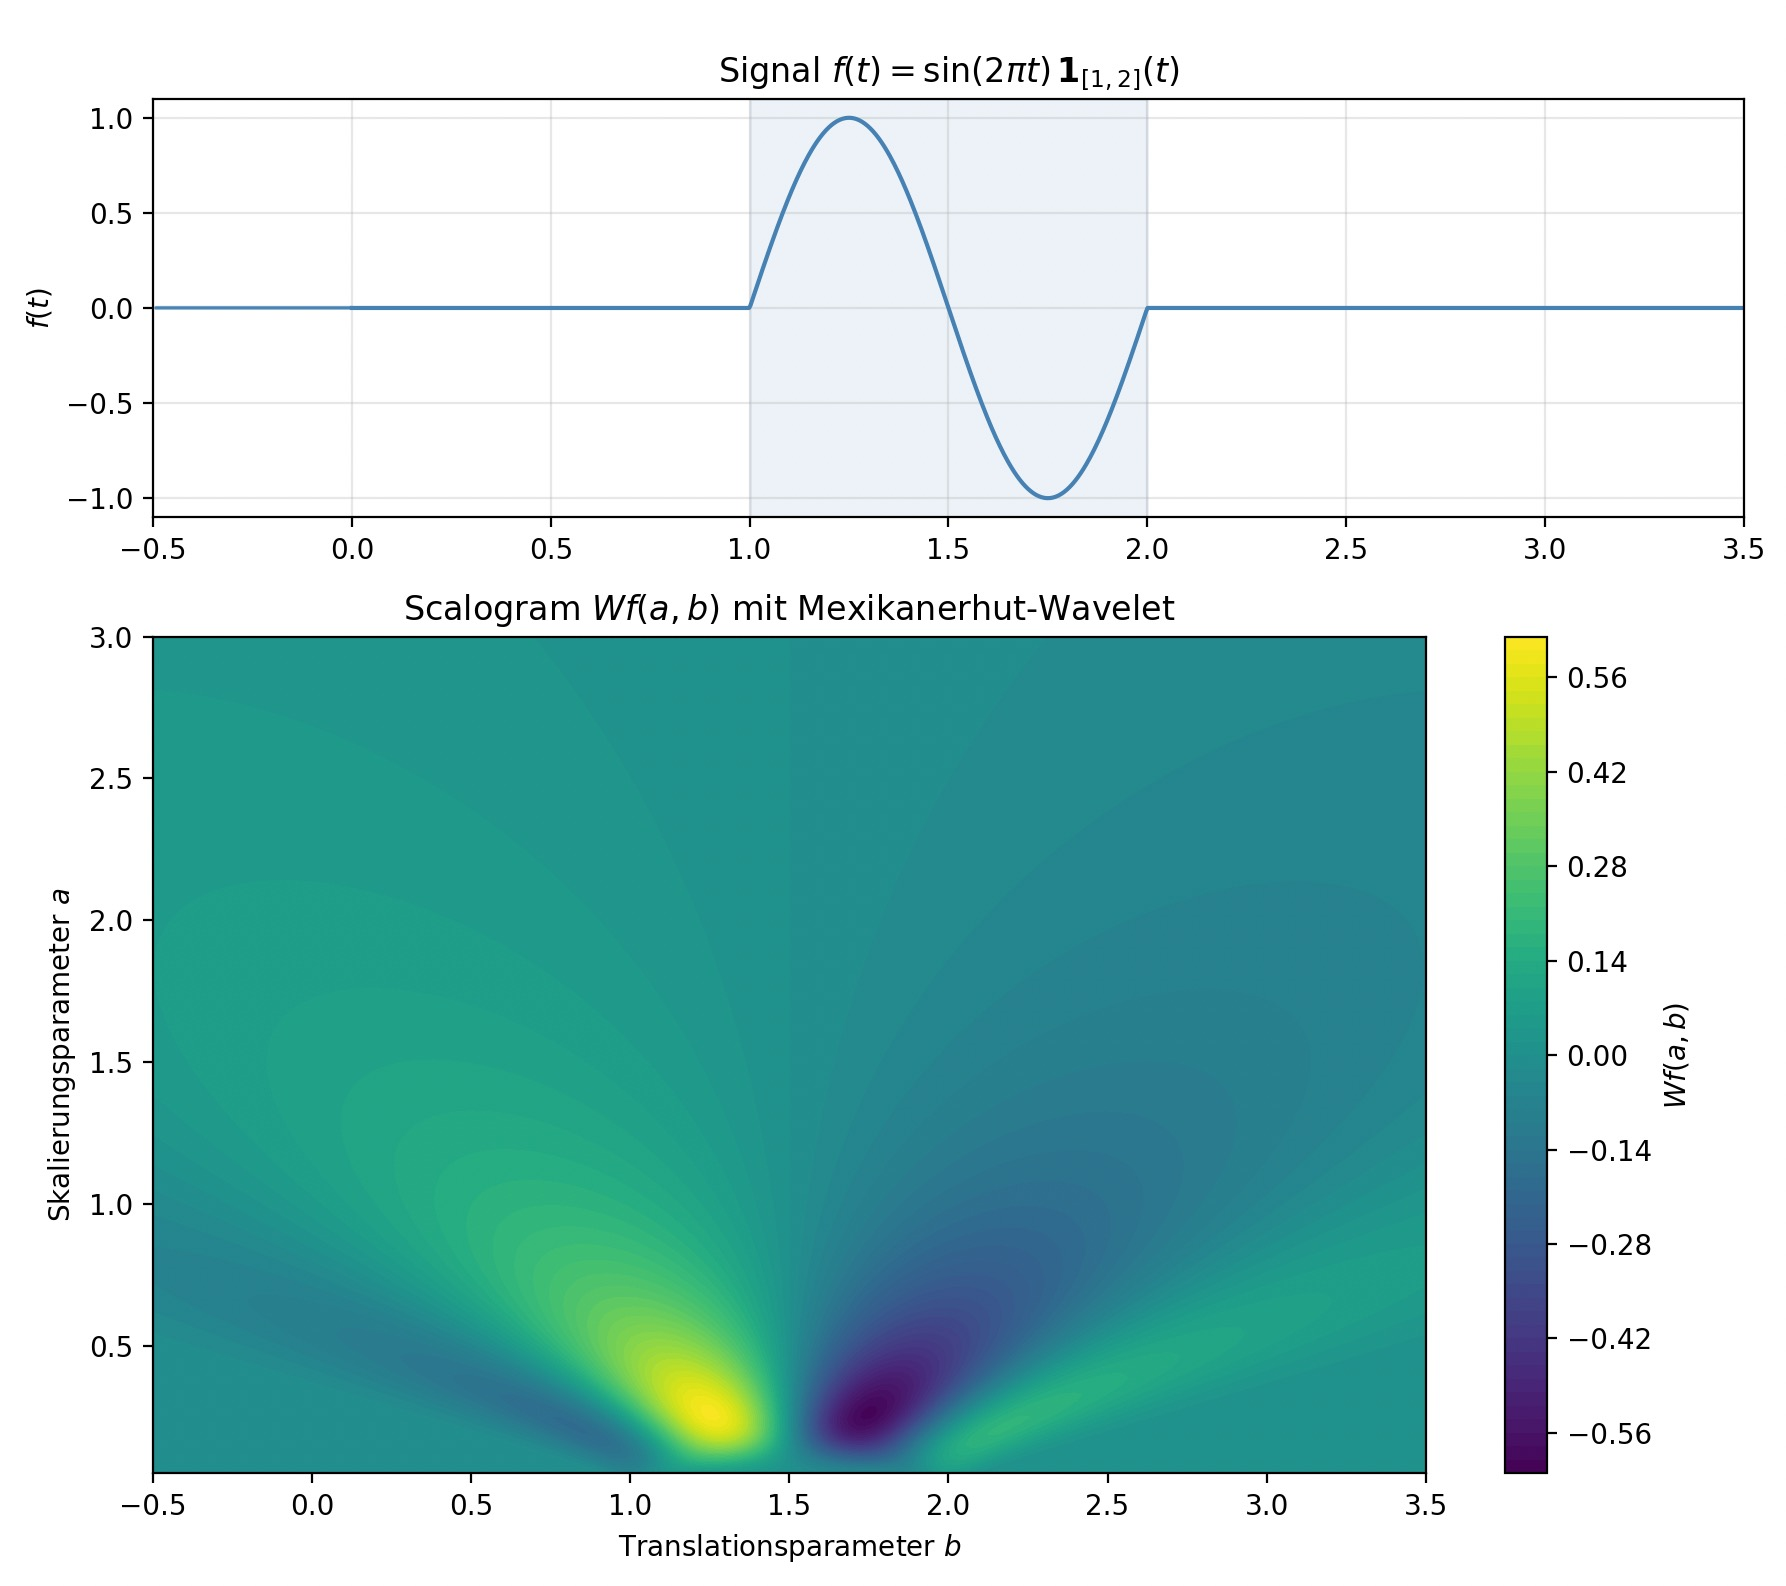
\includegraphics[width=\textwidth,keepaspectratio]{wavelettrafo_mexikanerhut_scalo.jpg}
      \caption{Skalogramm}
    \end{subfigure}\hfill
    \begin{subfigure}{0.55\textwidth}
      \centering
      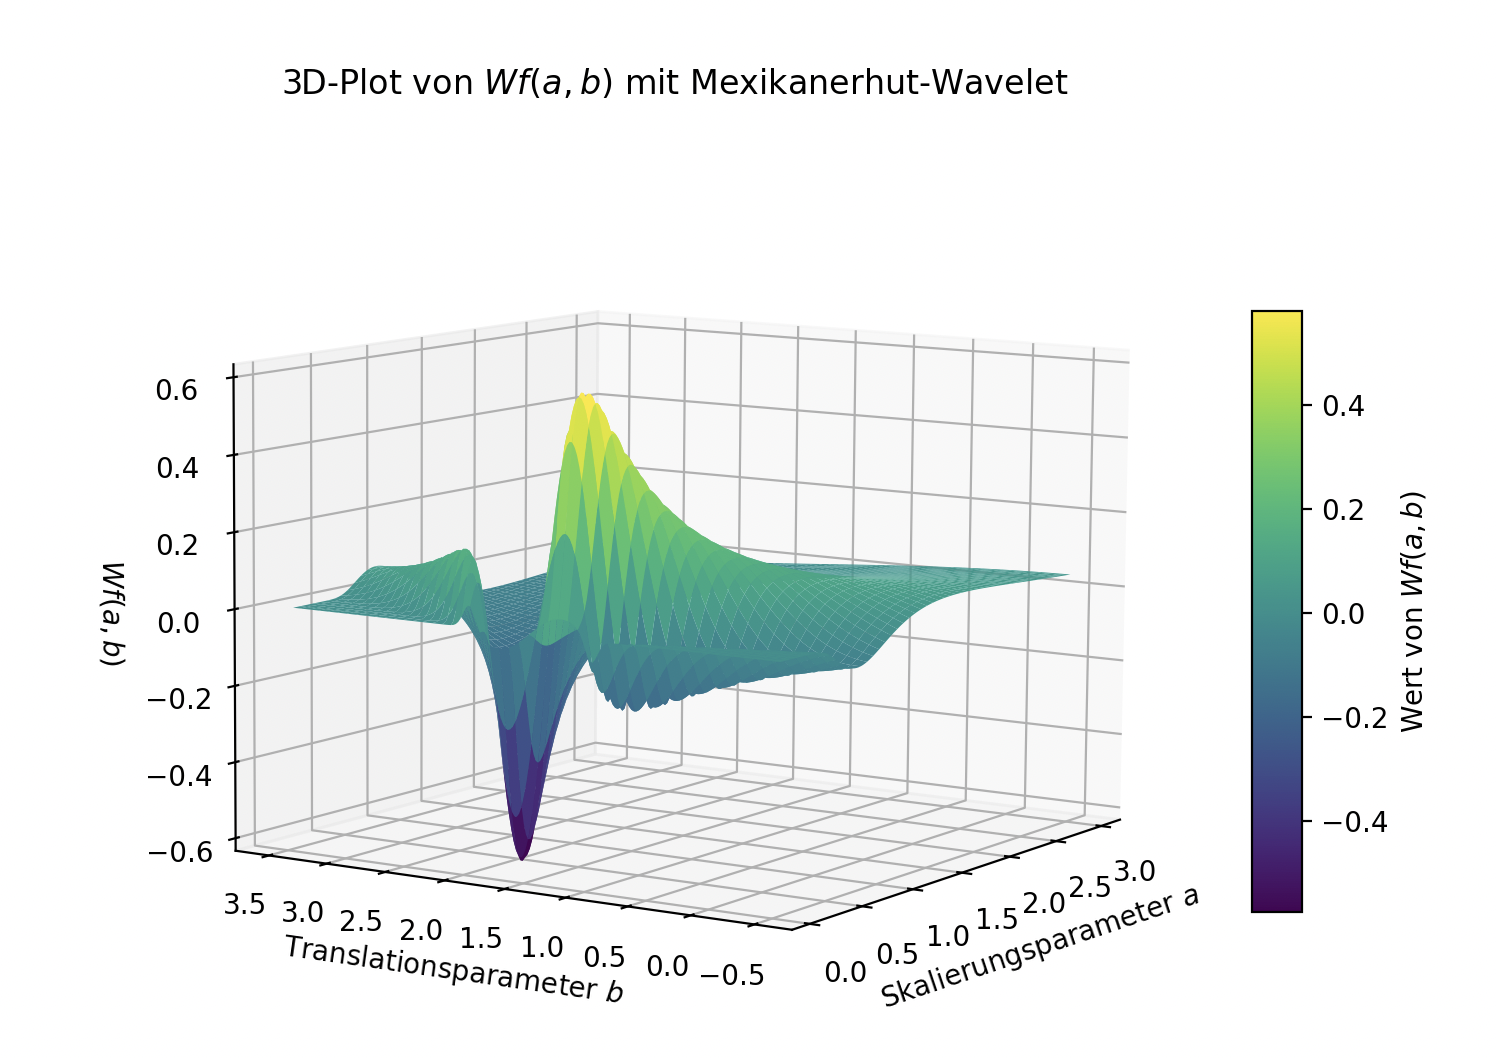
\includegraphics[width=\textwidth,keepaspectratio]{wavelettrafo_mexikanerhut_3d.png}
      \caption{3D-Plot}
    \end{subfigure}
    \caption{Visualisierung der Wavelet-Transformation der Funktion $f$ mit Mexikanerhut.}
    \label{fig:wavelettrafo_mexikanerhut}
  \end{figure}

  Das Skalogramm zeigt die Werte von $Wf(a,b)$ als Farbcodierung, während der 3D-Plot die
  Werte als Höhe einer Oberfläche darstellt.

  Man erkennt bei $b \approx 1{,}25$ ein Maximum und bei $b \approx 1{,}75$ ein Minimum,
  beide bei einer Skala von $a \approx 0{,}3$.

  Betrachtet man die folgende Abbildung~(4.?) und erinnert sich an die Definition der
  Wavelet-Transformation:
  \[
    Wf(a,b) = \langle f, \psi_{a,b} \rangle,
  \]

  \begin{figure}[htbp]
    \centering
    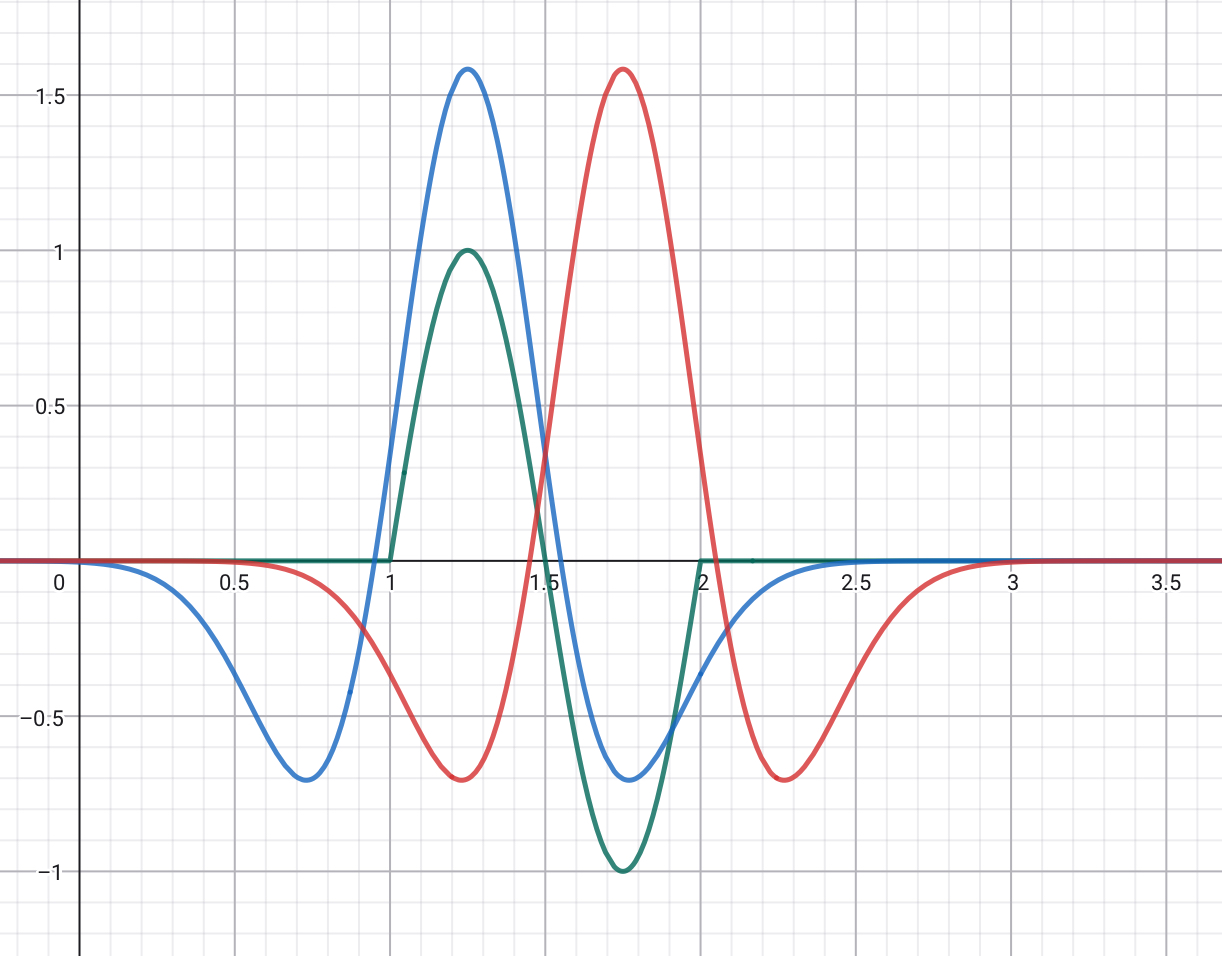
\includegraphics[width=0.5\textwidth]{waveletrafo_minmax.jpg}
    \caption{Das Signal $f$ dargestellt in grün, sowie die skalierten und verschobenen
      Versionen des Mexikanerhut-Wavelets $\psi_{0.3,1.25}$ in blau und $\psi_{0.3,1.75}$
      in rot.}
  \end{figure}

  so wird ersichtlich, warum die Extremstellen an diesen Stellen auftreten: Die Ähnlichkeit des
  Signals $f$ mit den Waveletfunktionen $\psi_{0.3,1.25}$ bzw.\ $\psi_{0.3,1.75}$ ist an
  diesen Stellen maximal bzw.\ minimal.
  Für größere Skalen $a$ ist die Ähnlichkeit gering, da das Wavelet zu breit ist, um die
  lokalen Strukturen des Signals zu erfassen.
  Für $b$ außerhalb des Intervalls $[1,2]$ ist die Ähnlichkeit ebenfalls gering, da das
  Signal dort null ist und somit keine Übereinstimmung mit dem Wavelet vorliegt.

  Insgesamt zeigt dieses Beispiel, wie die Wavelet-Transformation lokale Strukturen in einem
  Signal erfassen kann, indem sie die Ähnlichkeit mit skalierten und verschobenen Versionen
  eines Mutterwavelets misst.
\end{beispiel}

Ein weiteres wichtiges Wavelet das vorallem später beim Entfernen des Rauschens der EKG-Signale wichtig wird, ist das db4-Wavelet 

Dieses ist definiert durch 

\[
\psi_{db4} := blahblah
\]
 
\textcolor{blue}{hier bitte db4 gescheit definieren..... vll macht das auch erst später sinn....}
\textcolor{blue}{noch komplizierteres signal? - ampel?}
\textcolor{blue}{eventuell vergleich db4/ mexikanerhut}


  % ------------------------------------------------------------
  \subsection{Umkehrformel der Wavelet-Transformation}
  % \cite[Section 3.3]{blatterWaveletsEinfuhrung2003}
  
  
  \textcolor{red}{In unserem Anwendungskontext - der Bereinigung eines EKGs von Rauschen - benötigen wir 
  unser Signal $f$ im Endeffekt wieder aus $\mathcal{W}f(a,b)$ zurückgewinnen. 
  Hierfür müssen wir also die Wavelettransformation wieder rückgängig machen. 
  Grundlage dafür ist die folgende Plancherel-artige Formel.
  In der klassischen Fourier-Analysis besagt der Satz von Plancherel, dass die Fourier-Transformation die L2 norm erhält.
  Blatter zeigt hier das Äquivalent für die Wavelet-Transformation.}

  \begin{theorem}[Plancherel-Formel für die CWT] \cite[Satz 3.3, S. 62]{blatterWaveletsEinfuhrung2003}
   Sei $\psi$ ein zulässiges Wavelet nach Definition 2 und
   $\mathcal{W}$ die zugehörige Wavelet-Transformation nach Definition 4. Dann gilt für beliebige
   $f, g \in L^2(\mathbb{R})$
   \[
     \langle \mathcal{W}f, \mathcal{W}g \rangle_H \;=\; C_\psi \, \langle f, g \rangle ,
   \]
   wobei
   \[
     C_\psi := 2\pi \int_{\mathbb{R}^*} \frac{|\hat\psi(t)|^2}{|t|}\, dt
   \]
   die Zulässigkeitskonstante aus Definition 2 (2) von $\psi$ ist und $H := L^2(\mathbb{R}^2_-, d\mu)$
   mit dem Maß $d\mu = \frac{da\,db}{|a|^2}$.

   WAS IST DIESES MAß UND WAS IST R2- MUSS IN GRUNDLAGEN!!
  \end{theorem}
   
  \begin{proof}
   \textcolor{blue}{HIER KANN MAN DEN BEWEIS AUS BLATTER S.61-63 EINFÜGEN (PLANCHEREL
   + FUBINI + SUBSTITUTION). EVTL. NUR SKIZZIEREN, DA TECHNISCH.}
  \end{proof}
  
  \begin{bemerkung} NOCH BISSCHEN INTUITIVER ERKLÄREN...
   Die Formel besagt, dass die CWT bis auf den Faktor $C_\psi$ eine Isometrie
   zwischen $L^2(\mathbb{R})$ und einem Teilraum von $H$ ist. Diese Strukturerhaltung
   ist der entscheidende Grund, warum sich die CWT überhaupt umkehren lässt: Eine
   Isometrie ist injektiv und ihr Bild lässt sich (im richtigen Sinne) wieder
   zurückrechnen. WANN GENAU KANN MAN DAS JETZT UMKEHREN MUSS MAN GLEICH NOCH GENAUER ERKLÄREN....
  \end{bemerkung}

  Um aus der Plancherel-Formel eine punktweise Rekonstruktionsformel zu gewinnen,
  benötigen wir ein Regularisierungslemma.
 
  \begin{lemma}{Regularisierung durch Gauß-Glättung} \cite[S.~66, Section~3.3]{blatterWaveletsEinfuhrung2003}

   Sei die Dichte der Normalverteilung mit der Standardabweichung $\sigma > 0$ gegeben durch 

   \[
   g_\sigma(t)
   :=
   \frac{1}{\sqrt{2\pi}\,\sigma}
   \exp\!\left(-\frac{t^2}{2\sigma^2}\right).
   \]
   
   Ist $f \in L^1(\mathbb{R})$ und an der Stelle $x$ stetig, so nähert sich die Faltung von
   $f$ mit $g_\sigma$ für $\sigma \to 0^+$ dem Funktionswert von $f$ an. 
   Es gilt also   
   \[
   \lim_{\sigma \to 0^+} (f * g_\sigma)(x) = f(x).
   \]

  \end{lemma}  

  \begin{proof}
   BEWEIS SIEHE BLATTER S.66
   \textcolor{blue}{STANDARD-EPSILON-H-ARGUMENT, EVTL. WEGLASSEN ODER NUR ZITIEREN -- IST
   EIGENTLICH KLASSISCHE ANALYSIS UND NICHT WAVELET-SPEZIFISCH.}
  \end{proof}

  Mit diesem Lemma und der Plancherel-Formel erhalten wir die zentrale
  Umkehrformel der CWT:

  \begin{satz}[Umkehrformel der CWT] WAS SIND DEN JETZT DIE KONKRETEN VORRAUSSETZUNGEN??
   Unter geeigneten Voraussetzungen an $f$ und $\psi$ gilt in jedem Stetigkeitspunkt 
   $x$ von $f$:
   \[
     f(x) \;=\; \frac{1}{C_\psi} \int_{\mathbb{R}^2_-} \mathcal{W}f(a,b)\,
     \psi_{a,b}(x) \, \frac{da\,db}{|a|^2} .
   \]
  \end{satz}
   
  \begin{proof}
   \textcolor{blue}{IDEE: IN DER PLANCHEREL-FORMEL $g := T_x g_\sigma$ SETZEN, MIT
   $(f * g_\sigma)(x) = \langle f, T_x g_\sigma\rangle$ KOMBINIEREN UND
   $\sigma \to 0$ MIT REGULARISIERUNGSLEMMA. DETAILS EVTL. NUR ANDEUTEN, SIEHE
   BLATTER S.66-67.}
  \end{proof}

  \begin{bemerkung}[Intuition]
   Diese Formel ist das Analogon zur Fourier-Rücktransformation: Während die
   Fourier-Synthese ein Signal als Überlagerung von Sinus- und Kosinusschwingungen
   $e^{i\xi t}$ mit den Fourier-Koeffizienten $\hat f(\xi)$ als Gewichten
   rekonstruiert, setzt die CWT-Umkehrformel $f$ als (kontinuierliche) eine Überlagerung (Superposition?)
   der verschobenen und skalierten Wavelets $\psi_{a,b}$ zusammen, gewichtet mit den
   Wavelet-Koeffizienten $\mathcal{W}f(a,b)$.
   
   \textcolor{blue}{HIER VLLT NOCH EINEN SATZ ZUR EKG-ANWENDUNG: DIE COEFFICIENTEN
   WF(A,B) SIND GENAU DIE GRÖSSEN, DIE BEIM DENOISING (THRESHOLDING) VERÄNDERT
   WERDEN -- ANSCHLIESSEND LIEFERT DIESE FORMEL (BZW. IHRE DISKRETE ENTSPRECHUNG,
   SIEHE KAPITEL 4) DAS REKONSTRUIERTE, GEGLÄTTETE SIGNAL.}
  \end{bemerkung}
  
  %\begin{bemerkung}[Varianten]
  % Beschränkt man sich auf reellwertige oder symmetrische Wavelets $\psi$ (was z.B.
  % für das Mexican-Hat-Wavelet gilt), so genügt es, nur Skalen $a > 0$ zu
  % betrachten ($\mathbb{R}^2_>$ statt $\mathbb{R}^2_-$). Zudem kann man zur Analyse
  % und zur Synthese verschiedene Wavelets $\psi$ und $\chi$ verwenden, sofern die
  % Kreuz-Admissibilitätskonstante $C_{\psi\chi}$ existiert.
  % \textcolor{blue}{BILD HIER: SKIZZE WF(A,B) -> THRESHOLDING -> REKONSTRUKTION,
  % EVTL. ALS DIAGRAMM/FLOWCHART}
  %\end{bemerkung}


  

  % ------------------------------------------------------------
  \subsection{Diskrete Wavelet-Transformation (DWT)}
  % \cite[ch. 3, p. 53--106]{daubechiesTenLecturesWavelets2006}
  % \cite[Section 4]{blatterWaveletsEinfuhrung2003}

  \subsubsection{Motivation der Diskretisierung: Redundanz und das dyadische Gitter}
  \begin{itemize}
    %\item CWT: Parameter $a \in \mathbb{R}^*$, $b \in \mathbb{R}$ → unendlich viele Werte,
    %  auf dem Computer nicht realisierbar
    %  \cite[ch.\,3, p.\,53--106]{daubechiesTenLecturesWavelets2006}
    %\item EKG-Signal bereits diskret (z.\,B. 360\,Hz beim MIT-BIH Datensatz)

    \item CWT massiv redundant: benachbarte $(a,b)$-Werte liefern fast identische Information

    \item -> das ursprüngliche signal ist 1d das ergebnis der wavelettrafo 2d 

    \item -> $W(a,b)$ hängt von skalierung $a$ und Verschiebung $b$ ab. 

    \item -> hier DEFINITION FRAME \cite[S.87,88]{blatterWaveletsEinfuhrung2003}

    \item -> Motiviation: Unterschied Frame vs BASIS

    \item -> Wavelets bilden Frame: \cite[S.90, 91 / Satz 4.8]{blatterWaveletsEinfuhrung2003}

                                    \cite[S.94 / Satz 4.10]{blatterWaveletsEinfuhrung2003}


    \item -> weil a und b aus R sind hat man jetzt quasi doppelt so viele informationen 

    \item -> eng benachtbarte punkte von W enthalten quasi die gleiche information -> unnötig

    \item -> muss dann bei der Rücktransformation wieder über alle a und alle b zurückintegrieren 
    dabei integriert man die rednundaten informationen wieder heraus

    \item -> ist für datenverarbeitung verschwendung 

    \item -> deswegen stellt man sich die frage welche werte für a und b kann ich weglassen, 
    welche sind wichtig damit ich bei der transformation keine informationen verliere

    \item Idee: Gitter von $(a,b)$-Werten statt kontinuierlicher Parameter

    \item -> "Wie weit muss ich auf der a-Achse und der b-Achse springen (Abtastung), damit 
    die Wavelets gerade so weit auseinanderliegen, dass sie sich nicht mehr gegenseitig 
    behindern und die lineare Abhängigkeit verschwindet?"

    \item -> antwort dydadisches gitter 

    \item Standardwahl (dyadisches Gitter):
      \[
        a = a_0^m, \quad b = n \cdot b_0 \cdot a_0^m, \quad m,n \in \mathbb{Z}
      \]
      mit $a_0 = 2$ (Oktaven), $b_0 = 1$
    \item Intuition: bei grober Skala weniger Verschiebungen nötig (Wavelet bereits breit)
    \item Zentrale Frage: Geht durch Diskretisierung Information verloren? → Frame-Begriff
    -> ziel der DWT: orthorormale Basis von $L^2$ finden, und zwar aus wavelets 
  \end{itemize}

  \subsection{Die Multiresoltionsanalyse (MRA)}
  -> der hintergrund warum das dyadische Gitter eine orthornormalbasis bildet...

  -> motivation - wie funktionert zerlegung

  -> definition $V_j$ und $W_j$

  -> erklärung warum dann dyadisches Gitter orthonormalbasis liefert


  MRA zerlegt $L^2$ in eine Kette von ineinander verschachtelten Unterräumen $V_j$ 
  (mit $j \in \mathbb(Z)$ die Aufölsungsstufe darstellt)

  Es gilt 

  $V_0$ ist ein grobes Sieb,

  $V_1$ ist ein feineres Sieb,

  $V_2$ ist ein ncoh feineres Sieb.

  Es gilt die Verschachtelung: 

  $\cdots \subset V_{-1} \subset V_0 \subset V_1 \subset \cdots \subset L^2(\mathbb(R))$

  -> bei blatter andersrum...... \cite[S. 106]{blatterWaveletsEinfuhrung2003}
  Das heisst: alles was im groben raum $V_0$ dargestellt werden kann, kann 
  auch im feineren raum $V_1$ dargestellt werden... Wenn j gegen unendlcih geht kann man 
  jedes beliebiges Signal perfekt beschreiben.

  Wenn $V_0 \subset V_1$ echte teilmenge weil $V_1$ mehr details hat enthält als $V_0$
  dann muss es einen Raum geben der genau diesen Unterschied beschreibt.
  Nennen wir $W_0$, dieser Raum ist das orthogonlae Komplement von $V_0$ in $V_1$:

  \cite[S. 108 / Satz 5.1]{blatterWaveletsEinfuhrung2003}
  $V_1 = V_0 \otimes W_0$

  wobei $\otimes$, dydadischwes Produkt/direkte Summe, bedeutet, dass man jede Funktion aus 
  $V_1$ so aufteilen kann: ein groben anteil aus $V_0$ und einen Detailteil aus $W_0$

  Man kann das weiter machen sodass man dann jede funktion aus $L^2$ darstellen kann
  als ...

  also: $L^2(\mathbb(R))= V_0 + W_0 \otimes W_1 \otimes W_2 \otimes \cdot$
 
 
 
 \subsection{Skalierungs- und Waveletfunktion (Father vs Mother Wavelet)}

 -> Definition Father Wavelet Pj bei blatter \cite[S. 109]{blatterWaveletsEinfuhrung2003} \cite[S. 110 / Section 5.2]{blatterWaveletsEinfuhrung2003}
  \cite[S. 111 / Satz 5.3]{blatterWaveletsEinfuhrung2003}
 -> Unterschied Mother Wavelet TIEFPASS UND HOCHPASSFILTER \cite[S. 124]{blatterWaveletsEinfuhrung2003}
 -> vergleich mit beispiel \cite[S. 127]{blatterWaveletsEinfuhrung2003}
 -> FW basis für V räume und 
 -> MW basis für W detailräume \cite[S.122 / Satz 5.12, 5.13]{blatterWaveletsEinfuhrung2003}


 
 \subsection{Mallat-Algorithmus}

 -> quasi implementierung der MRA in der Praxis
 Wie die Koeffizienten der Skalierungsgleichung zu Tiefpass- (h) und 
 Hochpassfiltern (g) werden. Das Prinzip des Downsamplings (↓2).

 \subsection{Die inverse DWT (IDWT)}

 -> Wie man aus den Approximations- und Detailkoeffizienten durch Upsampling 
 (↑2) und Synthese-Filter das Signal fehlerfrei rekonstruiert.



% \subsubsection{Frames – Definition und Eigenschaften}
%  % \cite[Section 4, S. 79--88]{blatterWaveletsEinfuhrung2003}
%  % \cite[Preliminaries S. xix]{daubechiesTenLecturesWavelets2006}
%  \begin{itemize}
%    \item \textbf{Vereinfachte Definition}
%      \cite[Section~4, S.\,79]{blatterWaveletsEinfuhrung2003}:
%      \begin{itemize}
%        \item Frame = Kollektion $(a_i \mid i \in I)$ von Vektoren in Hilbertraum $X$,
%          so dass kein $x \in X$ auf allen $a_i$ senkrecht steht
%        \item Im unendlichdimensionalen Fall nicht trivial zu sichern
%        \item Frames müssen nicht linear unabhängig oder orthonormal sein → im Allgemeinen redundant
%      \end{itemize}
%    \item \textbf{Geometrische / algebraische Definition}
%      \cite[Section~4, S.\,82]{blatterWaveletsEinfuhrung2003}:
%      \begin{itemize}
%        \item Operatordefinition: $T\colon X \to \ell^2(I)$, $(Tx)_i := \langle x, a_i \rangle$
%        \item $(a_i)$ ist Frame $\Leftrightarrow$ es gibt $B \geq A > 0$ mit
%          \[
%            A\|x\|^2 \leq \|Tx\|^2 \leq B\|x\|^2 \quad \forall x \in X
%          \]
%        \item $A$, $B$: untere / obere Framekonstanten
%        \item Straffer (tight) Frame: $A = B$ → $T$ im Wesentlichen isometrisch,
%          $G = A \cdot \mathrm{id}_X$ (Gram-Operator)
%      \end{itemize}
%    \item \textbf{Allgemeine (Maßraum-)Definition}
%      \cite[Section~4, S.\,87--88]{blatterWaveletsEinfuhrung2003}
%      \cite[Preliminaries, S.\,xix]{daubechiesTenLecturesWavelets2006}:
%      \begin{itemize}
%        \item $X$: komplexer (unendlichdimensionaler) Hilbertraum
%        \item $M$: Maßraum mit Maß $\mu$ und $\sigma$-Algebra $\mathcal{F}$;
%          ermöglicht $Y := L^2(M,\mu)$
%        \item Familie $h_\cdot = (h_m \mid m \in M)$, $h_m \in X$
%        \item Analysisoperator: $Tf(m) := \langle f, h_m \rangle$
%        \item Quantifizierung der Information:
%          $\|Tf\|^2 := \int_M |Tf(m)|^2\,d\mu(m)$
%        \item $(h_m)$ ist Frame, falls:
%          \begin{enumerate}
%            \item $Tf$ ist $\mu$-messbar für alle $f \in X$
%            \item $\exists B \geq A > 0$: $A\|f\|^2 \leq \|Tf\|^2 \leq B\|f\|^2$
%          \end{enumerate}
%        \item Obere Schranke $B$: $T$ ist beschränkter Operator $X \to Y$
%        \item Untere Schranke $A$: $T$ ist injektiv → kein Informationsverlust
%      \end{itemize}
%    \item Verbindung zur DWT: diskrete Waveletfamilie $(\psi_{m,n})$ soll Frame in $L^2(\mathbb{R})$ sein
%  \end{itemize%}
%
%  \subsubsection{Riesz-Basen}
%  \begin{itemize}
%    \item TODO: Definition Riesz-Basis einfügen
%    \item Verhältnis zu Frames und ONB klären
%    \item Bedeutung für DWT: stabiles Darstellungssystem
%  \end{itemize%}
%
%  \subsubsection{Satz 4.10 (Frame-Garantie für DWT)}
%  % \cite[Theorem 4.10]{blatterWaveletsEinfuhrung2003}
%  \begin{itemize}
%    \item Aussage \cite[Theorem~4.10]{blatterWaveletsEinfuhrung2003}:
%      Sei $a_0 > 1$ (Zoomschritt) vorgegeben, $\psi$ zulässiges Wavelet
%      mit Parametern $a_0, b_0, C, A'$. Dann gibt es $b_0^*$, $B'$, $C'$, so dass:
%      \begin{itemize}
%        \item Für $b_0 < b_0^*$ ist $(\psi_{m,n} \mid m,n \in \mathbb{Z})$ ein Frame
%          mit Framekonstanten $A$, $B$
%      \end{itemize}
%    \item Konsequenz: \emph{numerische Stabilität} der DWT ist garantiert
%    \item Standardwahl $a_0 = 2$ (dyadisch) ist durch Satz gedeckt
%  \end{itemize%}%
%
%
%% ============================================================
%\section{Multiskalenanalyse (MRA)}
%% \cite[Section 5]{blatterWaveletsEinfuhrung2003}
%% \cite[Section 5]{daubechiesTenLecturesWavelets2006}
%% Ziel: algebraische Grundlage für schnelle Algorithmen + orthonormale Waveletbase%n
%
%  \begin{itemize}
%    \item Grundbild: Zerlegung von $L^2(\mathbb{R})$ in Leiter von Teilräumen
%      \cite[Section~5]{blatterWaveletsEinfuhrung2003}
%      \cite[Section~5]{daubechiesTenLecturesWavelets2006}:
%      \[
%        \ldots \subset V_{-1} \subset V_0 \subset V_1 \subset V_2
%        \subset \ldots \subset L^2(\mathbb{R})
%      \]
%    \item $V_j$ = Approximationen der Auflösung $2^j$:
%      \begin{itemize}
%        \item $V_0$: grobe Approximation (langsame Variationen)
%        \item $V_j$: feinere Approximation (doppelte Auflösung bei $j \to j+1$)
%      \end{itemize}
%    \item Schlüsselidee: Differenzraum / Detailraum $W_j$:
%      \[
%        V_{j+1} = V_j \oplus W_j
%      \]
%      $W_j$ enthält genau die Details, die beim Übergang $V_j \to V_{j+1}$ gewonnen werden
%    \item $W_j$ wird aufgespannt von den Wavelets $\psi_{j,k}$
%    \item EKG-Beispiel:
%      \begin{itemize}
%        \item $V_0$: Baseline-Verlauf
%        \item $W_0$: langsame Drift
%        \item $W_3, W_4$: QRS-Komplex (Skala der schnellen Strukturen)
%        \item $W_6, W_7$: hochfrequentes Rauschen
%      \end{itemize}
%    \item Denoising = gezieltes Nullsetzen oder Schwellwertanwenden auf bestimmte $W_j$
%  \end{itemize}
%
%  % ------------------------------------------------------------
%  \subsection{Axiomatische Definition der MRA}
%  % \cite[Section 5.1]{blatterWaveletsEinfuhrung2003}
%  % \cite[p. 129--136]{daubechiesTenLecturesWavelets2006}
%  \begin{itemize}
%    \item TODO: MRA-Axiome formal aufschreiben
%      \cite[Section~5.1]{blatterWaveletsEinfuhrung2003}
%      \cite[p.\,129--136]{daubechiesTenLecturesWavelets2006}
%      (Translationsinvarianz, Skalierungseigenschaft,
%      Vollständigkeit, Separabilität, Skalierungsfunktion $\phi$)
%  \end{itemize}
%
%  % ------------------------------------------------------------
%  \subsection{Skalierungsfunktion und Skalierungsrelation (Two-Scale-Relation)}
%  % \cite[Section 5.2]{blatterWaveletsEinfuhrung2003}
%  \begin{itemize}
%    \item Skalierungsfunktion $\phi$ zugehörig zu MRA
%      \cite[Section~5.2]{blatterWaveletsEinfuhrung2003}
%    \item Skalierungsrelation (Refinement equation):
%      \[
%        \phi(t) = 2 \sum_k h_k\, \phi(2t - k)
%      \]
%    \item $h_k$: Filterkoeffizienten (Tiefpass) → direkte Verbindung zu Mallat-Algorithmus
%    \item Analoges für Wavelet $\psi$:
%      \[
%        \psi(t) = 2 \sum_k g_k\, \phi(2t - k)
%      \]
%      mit Hochpassfilterkoeffizienten $g_k$
%    \item Zusammenhang $h_k$ und $g_k$: Konjugierte Quadraturfilter (CQF)
%      \begin{itemize}
%        \item TODO: Formel explizit eintragen
%      \end{itemize}
%  \end{itemize}
%
%  % ------------------------------------------------------------
%  \subsection{Wavelet-Raum}
%  \begin{itemize}
%    \item TODO: formale Konstruktion von $W_j$ aus $V_j$ und $V_{j+1}$ ausschreiben
%    \item Orthogonalität $V_j \perp W_j$
%    \item $\psi_{j,k}$ als ONB von $W_j$
%  \end{itemize}
%
%  % ------------------------------------------------------------
%  \subsection{Mallat-Algorithmus (schnelle Wavelet-Transformation)}
%  % \cite[Section 5.4]{blatterWaveletsEinfuhrung2003}
%  \begin{itemize}
%    \item Motivation: MRA liefert effizienten Berechnungsweg für DWT-Koeffizienten
%      \cite[Section~5.4]{blatterWaveletsEinfuhrung2003}
%    \item Zentrale Beobachtung: aus Skalierungsrelation folgt,
%      dass Koeffizienten der Ebene $j$ aus Ebene $j+1$ durch Filterung berechnet werden können
%    \item \textbf{Analysefilter (Vorwärtstransformation):} gegeben Koeffizienten auf Ebene $j+1$:
%      \begin{itemize}
%        \item $* h$ (Tiefpass) + Downsampling $\downarrow 2$ → Approximationskoeffizienten
%          auf Ebene $j$ ($V_j$)
%        \item $* g$ (Hochpass) + Downsampling $\downarrow 2$ → Detailkoeffizienten
%          auf Ebene $j$ ($W_j$)
%      \end{itemize}
%    \item \textbf{Rekursion:} Wiederholung auf dem Approximationsteil:
%%      Signal → (Approx$_1$, Detail$_1$) → (Approx$_2$, Detail$_2$) → $\ldots$
%%    \item Komplexität: $\mathcal{O}(N)$ → schneller als FFT mit $\mathcal{O}(N \log N)$
%%    \item \textbf{Synthesefilter (Rückwärtstransformation):}
%%      \begin{itemize}
%%        \item Upsampling $\uparrow 2$ + $* \tilde{h}$ und $* \tilde{g}$ (duale Filter) + Addition
%%      \end{itemize}
%%    \item Verbindung zum Haar-Beweis: Induktionsschritt im Vollständigkeitsbeweis
%%      ist im Wesentlichen ein Schritt des Mallat-Algorithmus
%%  \end{itemize}
%%
%
%% ============================================================
%\section{Konvergenzresultate}
%% Frage: Wann konvergiert Wavelet-Approximation, wie schnell?
%
%  % ------------------------------------------------------------
%  \subsection{$L^2$-Konvergenz der MRA-Approximation}
%  % \cite[Section 5.1, S. 108--109]{blatterWaveletsEinfuhrung2003}
%  \begin{itemize}
%    \item MRA erzeugt Folge von Projektionen
%      \cite[Section~5.1, S.\,108--109]{blatterWaveletsEinfuhrung2003}:
%      $P_j f = \sum_k \langle f, \phi_{j,k}\rangle\, \phi_{j,k}$
%    \item Grundresultat:
%      $\|f - P_j f\|_{L^2} \to 0 \quad (j \to \infty)$
%    \item Beweis: über MRA-Axiom $\overline{\bigcup_j V_j} = L^2(\mathbb{R})$
%    \item Bedeutung: Waveletentwicklung konvergiert immer in $L^2$; bei hinreichend feiner Auflösung
%      geht keine Information verloren
%  \end{itemize}
%
%  % ------------------------------------------------------------
%  \subsection{Lineare vs. nichtlineare Approximation}
%
%  \subsubsection{Lineare Approximation}
%  % \cite[Theorem 11.6]{mallatWaveletTourSignal1999}
%  \begin{itemize}
%    \item Definition: Approximation durch $m$ feste Skalenräume
%      (Indizes $(j,k)$ unabhängig von $f$)
%      \cite[Theorem~11.6]{mallatWaveletTourSignal1999}:
%      $f_m^{\mathrm{lin}} = \sum_{j \leq J} \sum_k \langle f, \psi_{j,k}\rangle\,\psi_{j,k}$
%    \item Fehlerrate für $f \in H^s$:
%      $\|f - f_m^{\mathrm{lin}}\|_{L^2} = \mathcal{O}(m^{-s/d})$
%    \item Problem: erfordert globale Regularität $s$ → schlecht für stückweise glatte Funktionen
%  \end{itemize}
%
%  \subsubsection{Nichtlineare Approximation}
%  % \cite[Section 11.5]{mallatWaveletTourSignal1999}
%  \begin{itemize}
%    \item Definition: Approximation durch die $m$ \emph{größten} Koeffizienten
%      (adaptiv, abhängig von $f$)
%      \cite[Section~11.5]{mallatWaveletTourSignal1999}:
%      $f_m^{\mathrm{nlin}} = \sum_{(j,k) \in \Lambda_m} \langle f, \psi_{j,k}\rangle\,\psi_{j,k}$,
%      \quad $|\Lambda_m| = m$
%    \item Fehlerrate: $\mathcal{O}(m^{-s/d})$ unter deutlich schwächeren Regularitätsannahmen
%    \item Funktionen, die nur stückweise glatt sind, werden viel effizienter erfasst
%    \item Intuition: Energie des Signals konzentriert sich in wenigen großen Koeffizienten
%      (Sparsity / Dünnbesetztheit)
%    \item \textbf{Überleitung zu EKG}:
%      \begin{itemize}
%        \item EKG außerhalb QRS-Komplex: relativ glatt
%        \item QRS-Komplex: kurze, scharfe lokale Struktur → Energie in wenigen großen Koeffizienten
%        \item Lineare Approx.\ (Fourier / MRA mit festen Skalen): viele Koeffizienten für QRS nötig
%        \item Nichtlineare Approx.\ (Wavelet-Thresholding): wenige Koeffizienten reichen aus
%        \item Theoretischer Unterbau für Donoho/Johnstone-Thresholding
%      \end{itemize}
%  \end{itemize}
%

%% ============================================================
%\section{Denoising / Signalverarbeitung mit der Wavelet-Transformation}
%% Roter Faden: Wie trenne ich Signal von Rauschen bei Überlagerung?
%
%  % ------------------------------------------------------------
%  \subsection{Signalmodell}
%  % \cite[S. 601--602]{mallatWaveletTourSignal1999}
%  % \cite[S. 26--27]{gacekIntroductionECGSignal2012}
%  \begin{itemize}
%    \item Beobachtetes Signal
%      \cite[S.\,601--602]{mallatWaveletTourSignal1999}
%      \cite[S.\,26--27]{gacekIntroductionECGSignal2012}:
%      $Y(t) = f(t) + \varepsilon(t)$
%    \item $\varepsilon$: weißes Rauschen, gleichmäßig über alle Frequenzen verteilt
%    \item Problem: Rauschen und Signal überlappen im Frequenzbereich vollständig
%    \item EKG-Kontext: $f$ = physiologisches Signal,
%      $\varepsilon$ = Elektrodenartefakte, Baseline-Drift, Muskelnoise
%  \end{itemize}
%
%  % ------------------------------------------------------------
%  \subsection{Lineare Baseline: Wiener-Filter}
%  % \cite[S. 605--608]{mallatWaveletTourSignal1999}
%  % \cite[Theorem 11.3]{mallatWaveletTourSignal1999}
%  % \cite[S. 610]{mallatWaveletTourSignal1999}
%  \begin{itemize}
%    \item Idee: Multiplikation jedes Frequenzkoeffizienten mit Gewicht $w_j \in [0,1]$
%      gemäß erwartetem Signal-Rausch-Verhältnis
%      \cite[S.\,605--608]{mallatWaveletTourSignal1999}
%    \item Theorem~11.3 \cite[Theorem~11.3]{mallatWaveletTourSignal1999}:
%      Wiener-Filter ist optimal (im linearen, quadratischen Sinn)
%      – aber nur wenn $f$ bereits bekannt
%    \item Limitation \cite[S.\,610]{mallatWaveletTourSignal1999}:
%      \begin{itemize}
%        \item Filter global: alle Koeffizienten einer Skala werden gleich behandelt
%        \item Bei lokal nicht-stationären Signalen (wie EKG mit QRS): zu viel oder zu wenig Glättung
%      \end{itemize}
%  \end{itemize}
%
%  % ------------------------------------------------------------
%  \subsection{Wavelet-Thresholding}
%  \begin{itemize}
%    \item Schlüsselbeobachtung:
%      \begin{itemize}
%        \item Rauschen verteilt sich gleichmäßig auf \emph{alle} Waveletkoeffizienten (klein, viele)
%        \item Signal konzentriert sich auf \emph{wenige, große} Koeffizienten
%      \end{itemize}
%    \item Strategie: kleine Koeffizienten $\approx$ Rauschen → nullsetzen;
%      große Koeffizienten $\approx$ Signal → behalten
%  \end{itemize}
%
%  \subsubsection{Hard Thresholding}
%  \begin{itemize}
%    \item Regel:
%      $\hat{c} = \begin{cases} c & |c| > \lambda \\ 0 & \text{sonst} \end{cases}$
%    \item Alles unter Schwelle $\lambda$: null; alles drüber: unverändert
%    \item Vorteil: einfach, erhält Signalspitzen
%    \item Nachteil: Diskontinuität bei $\lambda$ → Artefakte möglich
%  \end{itemize}
%
%  \subsubsection{Soft Thresholding}
%  \begin{itemize}
%    \item Regel:
%      $\hat{c} = \begin{cases} c - \lambda\,\mathrm{sign}(c) & |c| > \lambda \\ 0 & \text{sonst} \end{cases}$
%    \item Große Koeffizienten werden zusätzlich um $\lambda$ Richtung Null verschoben
%    \item Vorteil: stetig, glättet Artefakte an der Schwelle
%    \item In der Praxis oft besser als Hard Thresholding
%  \end{itemize}
%
%  \subsubsection{Donoho/Johnstone – Universeller Threshold}
%  % \cite[S. 623, Theorem 11.7]{mallatWaveletTourSignal1999}
%  \begin{itemize}
%    \item Problem: Woher kommt die Schwelle $\lambda$?
%    \item Universeller Threshold
%      \cite[S.\,623, Theorem~11.7]{mallatWaveletTourSignal1999}:
%      $\lambda^* = \sigma \sqrt{2 \log N}$
%      \begin{itemize}
%        \item $N$: Anzahl der Beobachtungen
%        \item $\sigma^2$: Rauschvarianz (in der Praxis zu schätzen, z.\,B. via MAD)
%      \end{itemize}
%    \item Theorem~11.7: $\lambda^*$ ist optimal im Minimax-Sinn
%      (minimiert schlimmstmöglichen Fehler über große Signalklasse)
%    \item Intuition: $\sigma\sqrt{2\log N}$ ist ca.\ das Maximum von $N$ unabhängigen
%      Gaußvariablen → alles Größere ist wahrscheinlich kein Rauschen
%  \end{itemize}
%
%  % ------------------------------------------------------------
%  \subsection{Schwellenwahl und SURE-Thresholding}
%  % \cite[S. 626--631]{mallatWaveletTourSignal1999}
%  % \cite[Theorem 11.9]{mallatWaveletTourSignal1999}
%  % \cite[S. 635--636]{mallatWaveletTourSignal1999}
%  \begin{itemize}
%    \item Universeller Threshold konservativ → überschätzt Rauschen gelegentlich
%    \item \textbf{SURE} (Stein's Unbiased Risk Estimate)
%      \cite[S.\,626--631]{mallatWaveletTourSignal1999}:
%      \begin{itemize}
%        \item Schätzt den Fehler direkt aus den Daten, ohne $f$ zu kennen
%        \item Wähle $\lambda$ als Minimierer des geschätzten Fehlers
%        \item Theorem~11.9 \cite[Theorem~11.9]{mallatWaveletTourSignal1999}:
%          mathematisch fundiert, datengetrieben
%        \item Passt sich automatisch ans Signal an → in der Praxis oft besser als universeller Threshold
%      \end{itemize}
%    \item Praktische Hinweise \cite[S.\,635--636]{mallatWaveletTourSignal1999}:
%      \begin{itemize}
%        \item TODO: Details aus Mallat ergänzen
%      \end{itemize}
%  \end{itemize}
%
%  % ------------------------------------------------------------
%  \subsection{Translationsinvariantes Thresholding}
%  % \cite[S. 632--633]{mallatWaveletTourSignal1999}
%  \begin{itemize}
%    \item Problem: DWT ist \emph{nicht} translationsinvariant
%      \cite[S.\,632--633]{mallatWaveletTourSignal1999}:
%      \begin{itemize}
%        \item Verschiebung des Signals um einen Abtastwert → völlig andere Koeffizienten
%        \item Hard/Soft Thresholding erzeugt sichtbare Artefakte (Gibbs-ähnliche Oszillationen)
%        \item Besonders störend bei EKG: künstliche Oszillationen im rekonstruierten Signal
%      \end{itemize}
%    \item Lösung: Mittelung über alle möglichen Verschiebungen des Signals
%      (Cycle Spinning / Translation Invariant Denoising)
%    \item Komplexität: $\mathcal{O}(N \log N)$ statt $\mathcal{O}(N)$, aber deutlich sauberere Ergebnisse
%    \item In der Praxis wichtig für klinische EKG-Analyse
%  \end{itemize}


\chapter{Anwendung auf EKG-Signale}
%%%%%%%%%%%%%%%%%%%%%%%%%%%%%%%%%%%%%%%%%%%%%%%%%%%%%%%%%%%%%%%%%%%%%%%%%%%%%%%%%%%%%%%%%%%%%%%%%%%%%%%%%%%%
\section{Datensets und Vorbereitung}

Charakteristika und Störeinflüsse von EKG Signalen
Kurze Beschreibung des Signals (Frequenzbänder der Spikes/QRS-Komplexe)
und typische Artefakte (Baseline-Wandern durch Atmung, hochfrequentes Muskelrauschen)

In welcher Form liegen daten vor? -> Herzzentrum, selbst konstruiertes EKG Signal..., MIT datenbank 

\section{Implementation of the Fourier Transform}
eigener phython code 
Was funktioniert hier nicht

\section{Implementation of the Wavelet Transform}
eigener phython code
Wie man das Signal zerlegt, Rauschen in bestimmten Detail-Koeffizienten identifiziert 
und mittels Hard- oder Soft-Thresholding (Schwellenwertverfahren) eliminiert, bevor man es wieder rekonstruiert.

Wie man die verbleibenden Detail-Koeffizienten nutzt, um die exakten Zeitpunkte von Herzschlägen (EKG) mathematisch
präzise zu lokalisieren.

\section{Results and discussion}

Vergleich der beiden Methoden
%%%%%%%%%%%%%%%%%%%%%%%%%%%%%%%%%%%%%%%%%%%%%%%%%%%%%%%%%%%%%%%%%%%%%%%%%%%%%%%%%%%%%%%%%%%%%%%%%%%%%%%%%%%%

\chapter{Conclusion}

zusammenfassung
%%%%%%%%%%%%%%%%%%%%%%%%%%%%%%%%%%%%%%%%%%%%%%%%%%%%%%%%%%%%%%%%%%%%%%%%%%%%%%%%%%%%%%%%%%%%%%%%%%%%%%%%%%%%%%
%%%%%%%%%%%%%%%%%%%%%%%%%%%%%%%%%%%%%%%%%%%%%%%%%%%%%%%%%%%%%%%%%%%%%%%%%%%%%%%%%%%%%%%%%%%%%%%%%%%%%%%%%%%%%%
% LITERATURBERZEICHNIS MIT BIBTEX --> MATHSCINET VERWENDEN
%%%%%%%%%%%%%%%%%%%%%%%%%%%%%%%%%%%%%%%%%%%%%%%%%%%%%%%%%%%%%%%%%%%%%%%%%%%%%%%%%%%%%%%%%%%%%%%%%%%%%%%%%%%%%%
%%%%%%%%%%%%%%%%%%%%%%%%%%%%%%%%%%%%%%%%%%%%%%%%%%%%%%%%%%%%%%%%%%%%%%%%%%%%%%%%%%%%%%%%%%%%%%%%%%%%%%%%%%%%%%

\bibliographystyle{alpha}
%\bibliographystyle{abbrv}
\bibliography{literature}

\end{document}
